\chapter{Photon Detector}
\label{ch:photon}
\section{Introduction}

\fixme{In our 2012 CDR we started each chapter with:  The scope of the (whichever) subsystem includes the design, procurement, fabrication, testing, delivery and installation of the mechanical and high voltage components of the (blah); followed by list of components -- see the TPC chapter. At this late date, not sure it's worth it...}
\fixme{Carlos: I have difficulty finding most of the numbers representing the expected performance of the photon detection system. Therefore the majority of my fixme's are related to this central question: where can we find the benchmarking for the PD?}


Liquid argon is an excellent scintillating medium. With an average
energy needed to produce a photon of 19.5~eV (at zero field) a typical
particle depositing 1~MeV in liquid argon will generate 40,000~photons
with a wavelength of 128~nm. At higher fields this will be reduced but
at 500~V/cm the yield is still about $\sim$20,000~photons per
MeV. Roughly 1/3 of the photons are promptly emitted after about 6~ns
while the rest are are emitted with a delay of 1100-1600~ns. LAr
is highly transparent to the 128~VUV photons with a Rayleigh
scattering length and absorption length of \fixme{Carlos:the latest result is 55 cm}95~cm and >200~cm
respectively~\cite{bib:gracearxiv}. The relatively large light yield makes the scintillation
process an excellent candidate for determination of $t_{0}$ for
non-beam related events. Detection of the scintillation light may also
be helpful in background rejection.

\section{Requirements and Goals}

\subsection{Beam-based physics}

There are no requirements for the beam-based physics program, as the
\fixme{Carlos: accelerator clock is better than machine clock}machine clock will provide a $t_{0}$ with roughly 10 $\mu$s
resolution. Given that the electron drift is 1.6 mm/$\mu$s the
uncertainty to the electron lifetime correction is small is %\fixme{when?Carlos: yes, when} the beam
timing is used. The photon system can be useful in determining the
$t_{0}$ of cosmic ray events and events from radiological decays as
well as giving a handle to the location of beam events in the LAr
volume with respect to fiducial boundaries. The impact of the LAr
scintillation light on the detector performance needs to be
determined,\fixme{Carlos:the negative at the beginning makes it sound strange, better move the not and rephrase it a bit: but it is expected that its role in reducing backgrounds
for the oscillation program will not introduce additional requirements to
the photon system design.}

\subsection{Proton Decay and Atmospheric Physics}

The photon detector system must provide the t$_0$ for non-beam related
physics channels if a correction for electron recombination during
drift is to be applied. The requirements for electronics and hadronic
energy resolution for the proton decay and the atmospheric neutrino
program are\fixme{Carlos: I can not find where these numbers come from $1\% / \sqrt{E(GeV)} \bigoplus 1\%$ and $30\% /
\sqrt{E(GeV)}$} respectively. With these resolutions the collected
charge must be accurately corrected for recombination. Therefore the
photon system must provide a $t_{0}$ for particles with >100 MeV with
>95\% efficiency in the fiducial volume of the detector.

\subsection{Low-energy Physics}

Supernova events will produce neutrinos down to about
$\sim$5~MeV. Studies have estimated the momentum resolution for 5 MeV
electrons to be 20\% using only TPC information and assuming a highly
efficient trigger and an electron lifetime of 5 ms. The impact of
various detector resolutions on the physics potential of LBNE has not
been studied in detail. At present there is no strong requirement that
the energy resolution %\fixme{Carlos: yes, we need must} %\must 
be better than 20\%, so no requirement on
the photon system trigger efficiency is set at this time. However it
is clear that if a detector design can be found, \fixme{clarify `detector design can be found'} \fixme{Carlos': I propose that we write: if a better detector design, with higher photon collection efficiency, can be found then the energy resolution could be significantly improved}
would greatly improve. A goal of the photon detection R\&D is to
develop a system with the lowest possible threshold for a reasonable
cost. At the %time of the %\fixme{Carlos: ok}
start of %\the final%\definitive design, a final decision as to the
configuration will need to be made based on cost and added physics
capability.

\subsection{Required Performance}

To achieve the physics goals in the previous section the performance
of the photon detection system must be understood. The prototype
readout electronics described in Section~\ref{sec_elec} have been
shown to detect the single photoelectron (p.e.) signals associated with the late
scintillation light but future versions may sacrifice this ability to
mitigate high channel costs %\fixme{Carlos: we should say how we intend to mitigate high channel costs}. It is assumed that the physics goals of
the photon detection system will be met using the prompt
scintillation light.

The performance, or overall photon collection efficiency, is given by
the following, where it is assumed only prompt light is collected:

\begin{equation}\label{eff_eqn}
\frac{N_{pe}}{MeV} = N_{128}\cdot \epsilon_{geom} \cdot \epsilon_{E} \cdot
\epsilon_{mesh} \cdot \epsilon_{conv} \cdot \epsilon_{capt}
\epsilon_{tran} \cdot \epsilon_{QE} 
\end{equation}

The efficiencies leading to the overall number of photo-electrons
collected by the photon detection system, $\frac{N_{pe}}{MeV}$, are given
in table~\ref{Table-Eff}.


\begin{cdrtable}[Individual photon collection efficiencies]{clcl}{example}
{Individual photon collection efficiencies}
 Factor & Description & Value & Comments \\ \toprowrule
   $\epsilon_{geom}$ & geometric acceptance & 0.0036 & historical
      average  \\ \colhline
      $\epsilon_{E}$ & field correction & 0.6 & 500~V/cm  \\ \colhline
      $\epsilon_{mesh}$ & TPC wire shadowing & .83 (30-150$^{\circ}$)
      & falls off sharply~\cite{HimmelMesh}  \\ \colhline
      $\epsilon_{conv}$ & TPB conversion & 1 & see
      ref.~\cite{bib:gehman}  \\ \colhline
      $\epsilon_{capt}$ & waveguide incident & 0.5 & about half
      converted photons\\ \colhline
      &  & & travel into waveguide  \\ \colhline
      $\epsilon_{tran}$ & waveguide transmission & TBD  & prototype
      dependent  \\ \colhline
     $\epsilon_{QE}$ & SiPM QE & .31  & SensL b-series  \\
\end{cdrtable}


Using Equation~\ref{eff_eqn} it is seen that to detect a
2~p.e. signal, likely to be discriminated from noise, the transport
efficiency is 1.2\%. Of course this value is very position-dependent,
as the geometric acceptance, wire shadowing and transport corrections
all depend on the location of the event. Figure~\ref{fig:photon_map}
shows the probability of (?)\fixme{} MeV energy deposition being detected in
the photon detectors. 

\begin{cdrfigure}[Probability of photon being detected in
  detectors when depositing energy]{photon_map}{Photon map giving the probability of photon being 
  detected in the photon detectors when depositing energy at map location. \fixme{(need
  general TPC cell map with better description)}}
  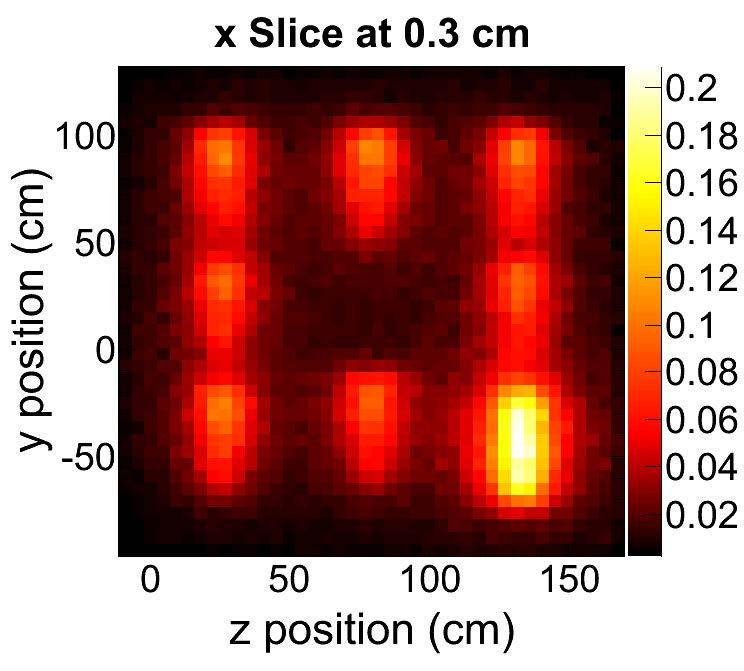
\includegraphics[width=0.4\textwidth]{35t_map.jpg}
\end{cdrfigure}


The TPC wire mesh shadowing is also quite location-dependent as photon
angles, relative to the wire plane, lead to rapid loss in transmission
below 30$^{\circ}$ and greater than 150$^{\circ}$. Lastly, the photon
detector paddles themselves can have position-dependent response to
incident photons due to the attenuation length of the waveguide. The
photon detector simulation, which is nearing stable operation, will be
able to better estimate the efficiencies coming from geometric
acceptance correction.

\subsection{General Considerations}

In the event that higher photon collection efficiencies can be
achieved it should be possible to improve the energy resolution of the
detector by adding the photon yield to the electron yield information.
However this requires several orders of \fixme{Carlos: magnitude} improvement in light
collection efficiency, so it is beyond the scope of the present design.

\section{Photon Detector Prototype Designs}

All designs considered for the photon detector have been based on the
use of wavelength-shifting coating, or bulk doping, of plastic
materials coupled to silicon photomultipliers (SiPMs). The reference
design utilizes a coated acrylic waveguide coupled to
SiPMs. This waveguide is described in Section~\ref{sec_bars}. Alternate waveguide designs, desribed in the following sections, have
been developed in an effort to optimize coverage, cost and attenuation length. 

\subsection{Cast or Bulk Doped Acrylic Bars}
\label{sec_bars}

The reference design for the photon detection system is based on light
guides that are coated with wavelength shifter. The 128-nm
scintillation photons from liquid argon interact with the wavelength
shifter on the light guide surface and \fixme{Carlos: peaking at 430-nm light is re-emitted} in
the bar.  The light guide channels the light to photodetectors at its
end.

A schematic drawing of a light guide with its photosensors is shown in
Figure~\ref{fig:WaveguideSketch}. The prototype light guides are bars
with a footprint 2.54 cm $\times$ 0.6 cm.  The concept is described in
Ref.~\cite{bib:MITbars}.

\begin{cdrfigure}[Schematic drawing of a light guide with its
      photosensors]{WaveguideSketch}{Schematic drawing of a light guide with its
      photosensors. The bars have embedded wavelength shifter (WLS),
      either TPB or bis-MSB. Three SiPMs collect the waveshifted
      photons that have been internally reflected to the bar's end. \fixme{Fuzzy at this size}}
    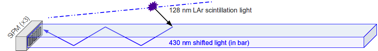
\includegraphics[width=.85\columnwidth]{cast-acryl-lightguide}
\end{cdrfigure}

The wavelength shifter converts incident VUV scintillation photons %striking it
to 430~nm photons inside the bar, with an efficiency of $\sim$50\% %of
for converting a VUV to an optical photon~\cite{bib:gehman}.  A fraction
of the waveshifted optical photons are internally reflected to the
bar's end where they are detected by SiPMs whose QE is well matched to
the 430-nm waveshifted photons. The light guides were made with one of
two wavelength shifters: the conventional TPB
(1,1,4,4-tetraphenyl-1,3-butadiene) and the less expensive alternative
bis-MSB (1,4-bis-(o-methyl-styryl)-benzene). Preliminary studies with
a VUV monochromator show that the two wavelength shifters compare
favorably in their waveshifting efficiency~\cite{bib:baptistaJINST}. A
testing program is currently underway to compare their relative
performance in liquid argon.

A team at Indiana University is studying prototype light guides made with three 
different technologies. These technologies are listed in
Table~\ref{tab:lightGuides}.

\begin{cdrtable}[Light guide technologies]{ c l  l }{lightGuides}
{Light guide technologies}
  Label & Light Guide Technologies \\ \toprowrule
  (a) & clear acrylic, dip-coated   \\ \colhline
      (b) & doped Eljen PVT light guide, dip-coated   \\ \colhline
      (c) & doped Eljen polystyrene light guide, dip-coated    \\ 
\end{cdrtable}



The clear acrylic bars (a) are made from blanks of commercially
available Lucite-UTRAN cast UVT acrylic sheet that has been laser-cut
and diamond-polished into bars of the proper size.  Lucite-UTRAN has
the longest attenuation length of the acrylics
tested~\cite{bib:mufsonJINST}.  The
Eljen\footnote{http://www.eljentechnology.com} bars (b and c) are commercial
light guides that are doped with J2 green fluor (equivalent to Y11).
Two types of light guides were purchased from Eljen.  The light
guides (b)  were fabricated from polyvinyl toluene (PVT); these are the
standard Eljen product EJ-280.  The quantum efficiency of the
fluorescent dopant in EJ-280 is 0.86, so the second shift in
wavelength does not markedly degrade the photon detector efficiency.
The light guides (c) were fabricated from polystyrene; these light
guides were ordered because PVT bars can craze if cooled too rapidly.
Although the PVT light guides may be brighter, no instance of crazing
has ever been observed in polystyrene light guides.

For the acrylic light guides, the WLS must be embedded in the plastic
at the bar's surface so that 128-nm scintillation photons can generate
optical 430-nm photons within the volume of the plastic.  Otherwise
the VUV photons will not be trapped by the light guide.  For the Eljen
bars, the wavelength shifter can either be embedded in the plastic, as
with the acrylic, or it can be deposited on a plate or film placed in
proximity to the light guides.  The J2 wavelength shifter then
converts the resulting 430-nm photons inside the light guides where
they are channeled to the photodetectors.

To embed the WLS at the surface of the light guides, a ``dip-coating''
process was developed at Indiana University.  Before the WLS was
applied to the acrylic bars, the bars were annealed at 80$^\circ$C for one
hour.  (The Eljen bars were not annealed.)  The WLS was dissolved in the
organic solvent\fixme{Carlos: dichlormethane (DCM)} (CH$_2$Cl$_2$).  For these waveguides
5~g of wavelength shifter was dissolved in 1,000~gm of DCM.  A
series of experiments showed that this concentration was optimum.  A
bar was first dipped into the WLS mixture for 15 seconds and then
removed.  It was then hung in the dark for at least two hours to dry.
Once dry, the ends of the bars were flycut.  Currently designs are
being fabricated that put an acrylic plate painted with WLS or a thin
film impregnated with WLS in front of the Eljen light guides.

In summer 2015 these designs will all be tested side-by-side at the
TallBo dewar facility at Fermilab under uniform, low-contamination
conditions.  In addition to the designs described above, these tests
will include photon detector designs from Colorado State University
and Louisiana State University.  This experiment will compare the
relative performance and the absolute efficiency for all designs
scaled to 1.5~m.

\subsection{Fiber-embedded Bulk Acrylic Plate}

%At LSU, Thomas Kutter and his team have 
The LSU team has developed a VUV photon detector
design for a large LAr detector that overcomes some of the
shortcomings of the present LBNE baseline \fixme{define `baseline' here; do you mean `reference design'?}%\fixme{Carlos: yes} photon detectors. The LSU
photon detector design allows for coverage of a very large area, thereby
increasing the geometrical acceptance of the photon detectors. The
number of required SiPMs and readout channels per unit detector area
covered with photon detection panels has been significantly reduced to
keep the overall cost for the photon detection system at or below the
present design while increasing the geometrical acceptance. % at the same time.

The photon detection system consists of a TPB-coated acrylic panel
with an embedded S-shaped wavelength shifting (WLS) fiber. The fiber
is read out by two SiPMs, which are coupled to either end of the fiber,
and serves to transport the light over long distances with minimal
attenuation. The double-ended fiber readout has the added benefit of
providing some position dependence to the light generation along the
panel by comparing relative signal sizes and arrival times in the two
SiPMs. Figure~\ref{fig:1-LSU} shows a drawing of the layout and a
photograph of a prototype photon detection panel in the test stand at
LSU.  The incoming 128-nm VUV Ar scintillation light will be converted
by the thin TPB layer on the acrylic panel and re-emitted with
wavelength peaking at 430~nm in an isotropic way. About 50\% of the
light %would be 
is emitted into the acrylic panel where some fraction will
be absorbed by the WLS fiber and converted to light with a peak
intensity of about 480 -- 500~nm. The green light exiting the fiber is
well matched to the peak photon detection efficiency of typical SiPMs.

\begin{cdrfigure}[LSU photon-detection panel]{1-LSU}{LSU photon-detection panel. Technical drawing of a $20"\times4.33"$ acrylic panel with embedded WLS fiber (left) and picture of a prototype in test set-up at LSU (right) with the same dimensions.}
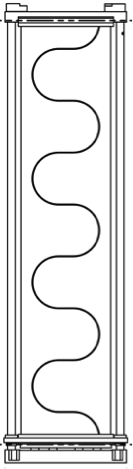
\includegraphics[width=0.25\linewidth]{LSU_panel_drawing.png}
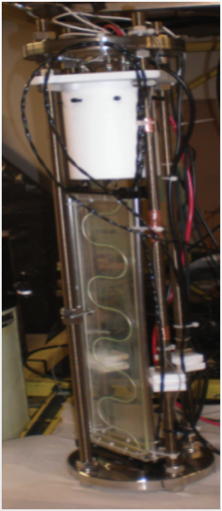
\includegraphics[width=0.45\linewidth]{LSU_panel_prototype.png}
\end{cdrfigure}

\fixme{Carlos: there is an asymmetry in the sections describing each of the designs: some of the subsections, like the ones describing the LSU and the CSU designs, go into details of the tests that were performed while the IU design receives no such treatment. I think this should be standardized for all designs}  

\subsection{LSU Photon detection panel production}

The photon detection panels are produced from 0.25-inch-thick
sheet UVT acrylic and cut to size. For a first series of prototypes
the acrylic panel dimensions were chosen to closely match the area of
four bars of the LBNE baseline \fixme{reference?} photon detection system.  The groove is
cut with a CNC mill in several passes to achieve good groove surface
quality, which is important for good light transmission from the bulk
acrylic to the fiber. The panels are dip coated with TPB and left to
dry prior to insertion of the WLS fiber. Panels with two and three
layers of fibers inserted and glued into the groove have been
produced. Fiber ends are cut and polished.  The resulting acrylic
panels are then inserted into a custom-made mechanical frame.% which was designed by David Warner at CSU. 
The end caps of the mechanical frame
house one SiPM on either end. The presently used $6\times6 mm^2$ active-area
SiPMs are spring-mounted to ensure good contact between the active area
and the fiber ends.  The leads of the SiPMs are connected to a small
Printed Circuit Board (PCB) %\fixme{define} %\fixme{Carlos: done} onto which $\sim$2-m-long twisted-pair coax cables are soldered to
supply the SiPM with a bias voltage and to read out signals. The other
cable ends are typically connected to pre-amplifiers before leading to
a DAQ system.  Components for the photon detection panels are
inspected at all stages of the manufacturing process for quality. Due
to the small number of panels produced to date, no quantitative quality
control parameters have been defined yet.  Proper connectivity of the
fully assembled units are tested in a setup at LSU using a LED
flasher. If LED light signals are seen, the panel is successively
immersed in gaseous argon (GAr) along with an alpha source. The
observation of %argon 
scintillation light originating from alpha
particles and cosmic rays penetrating the GAr volume allows for a
relatively quick quality-control check of a completed photon detector
at room temperature.

\subsection{Proof-of-Concept and Prototype Detector Results}

Several photon detector panels of $20 \times 4.33~in^2$ have been
produced and two have been tested in a LAr test stand at CSU. The
detectors submitted to the cold test have three and two embedded fibers,
respectively, but are otherwise produced in the same way. The data
taken in LAr included self-triggered alpha source scans as well as
cosmic runs with a muon hodoscope providing a trigger for near-vertical muons penetrating the LAr volume.
\paragraph{Alpha source runs:} The alpha source was placed at a distance of about 1~inch in front of the center line of the photon panel and moved to 20 different positions spaced about 1~inch apart from neighboring positions. At each position 5000 signal traces were recorded and measurements were repeated for three of the positions to check the reproducibility of the measured light yield. Figure~\ref{fig:2-LSU} shows results for both successively measured panels. The red and blue dots show the mean light yield values in units of p.e. (photo electron equivalents = no. of fired SiPM pixels) for the SiPM on the top and bottom end of the panel as function of source position. Green dots show the sum of both channels. The summed signals provide \fixme{indicate?} a very uniform detector response for the entire panel, independent of the alpha source position. The data also indicate good reproducibility for the doubly measured positions.
The three-fiber panel shows about 50\% more light when compared to the
two-fiber panel, which is in good agreement with expectations. It needs
to be pointed out that the LAr purity was not monitored and that
measurements for the two panels were performed sequentially after
refilling the dewar with LAr. However, the liquid argon for both
measurements came from the same batch, which motivates the assumption
that the purity for both measurements was very similar.

%
\begin{cdrfigure}[Light yield for the fiber LSU PD panels with alpha source in
  LAr]{2-LSU}{Light yield for the three (left) and two (right) fiber LSU photon
  detection panels in response to a 1-in distant alpha source in
  LAr. Red and blue symbols represent the mean light yield over 5000
  trigger events from a single SiPM each and green points represent
 the summed signal from both SiPMs.}
\resizebox{.48\textwidth}{!}{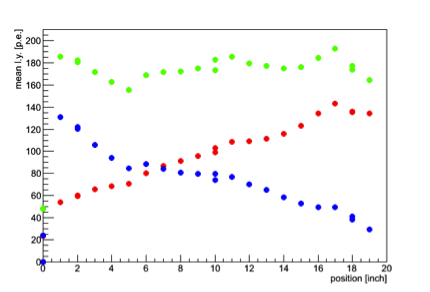
\includegraphics[width=0.45\linewidth]{LSU_panel_prototype1_ly-position.png}}
    \resizebox{.48\textwidth}{!}{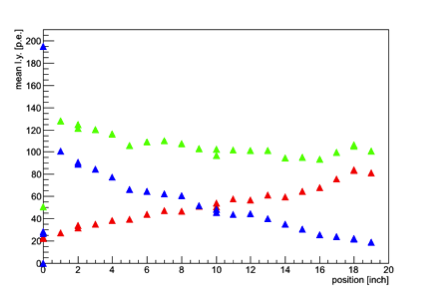
\includegraphics[width=0.8\linewidth]{LSU_panel_prototype2_ly-position.png}}
\end{cdrfigure}

%
\paragraph{Cosmic trigger runs:} Two $ 1" \times 10"$ wide scintillator counters were placed above and below the dewar to form a muon hodoscope and to select near-vertical muons traversing the LAr volume. The three-fiber LSU panel and one LBNL/Elgin Bis-MSB doped polystyrene bar of LBNE baseline dimensions and read out by three SiPMs were simultaneously inserted in the LAr. The setup allowed the study of the response of these photon detectors to scintillation light created by penetrating cosmic muons. A detailed quantitative comparison of the relative light yield was not possible with this setup due to large systematic uncertainties in the position dependence of the scintillation light generation by the triggering cosmic muons. A qualitative comparison of the detector responses, taken as the signal sum of three and two SiPMs for the Elgin bar and the LSU panel, respectively, shows comparable light yields as shown in Figure~\ref{fig:3-LSU}. 
        
%
%
\begin{cdrfigure}[Summed charge plots of SiPMs in response to muon hodoscope trigger]{3-LSU}{Scatter plot of the summed charge of three SiPMs coupled to the
 LBNL/Elgin Bis-MSB doped bar and the summed charge of two SiPMs for
 the three-fiber LSU panel in response to an external muon hodoscope
 trigger. The right plot shows a zoomed version of the left plot.}
   \resizebox{.48\textwidth}{!}{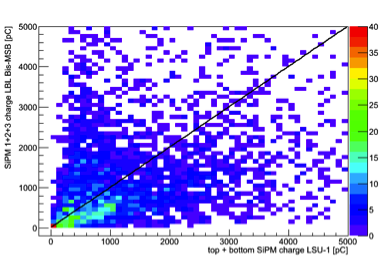
\includegraphics[width=0.45\linewidth]{LSU_panel_prototype_charge.png}}
   \resizebox{.48\textwidth}{!}{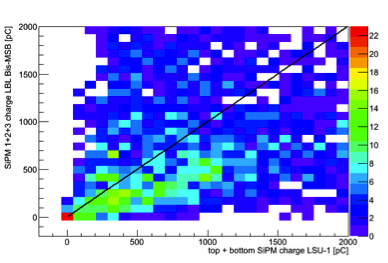
\includegraphics[width=0.8\linewidth]{LSU_panel_prototype_charge_zoom.png}}
\end{cdrfigure}

%

\subsection{R\&D Work in Progress and Present Plans }

After the construction and proof-of-principle test of the LSU-style
photon detection panels %we manufactured 
several 2.17-m-long and 110-mm-wide 
(=4.33") panels were manufactured to demonstrate the scalability of the design.  At
the time of writing, tests in the large LAr dewar at CSU are in
progress.  The team is performing alpha source scans and cosmic muon runs.
The alpha source scan runs are arranged such that the source
illuminates two photon detectors at the same time.  This setup
facilitates quantitative and relative light yield comparison between
different photon detector designs in the same LAr bath with a well-defined VUV light source.

Manufacturing and testing of wider panels is under consideration to
maximize the photon detector panel area in the DUNE LAr far
detector. The goal is to cover the entire anode plane assembly (APA)
area with photon detectors embedded into the APA frame.  Another
important measurement goal is to establish the energy threshold of the
photon detection panels. A study will be conducted for the photon
detectors presently installed in the 35t detector \fixme{reference sec in r\&d chap} using Michel
electrons. The 35t detector contains one of the three-fiber LSU photon
detection panels. In addition, performing alpha source runs in a well-controlled
and monitored LAr setup may provide information on the particle energy
threshold for observation of VUV scintillation light.  The measurement
of a photon detector panel's light yield as function of the source
distance is another key measurement to estimate the response and
sensitivity of the full photon detection system in a LAr
detector. Results will be useful to validate MC simulations.  We are
exploring options to perform these tests in the large dewar setup at
CSU or alternatively in the TallBo setup \fixme{ref?} at FNAL.

The TPB coating procedure of the acrylic panels has not yet been
optimized and improvements may be possible. A systematic
study is foreseen to identify parameters in the TPB dip and %alternatively 
in the
evaporation coating procedure to maximize the light yield of resulting
samples. These tests will be performed on small
$10\times10~\mathrm{cm}^2$ acrylic panels with a U-shaped embedded WLS
fiber.  On the software and analysis side, %we are in the process of improving our 
tools are being improved to study position dependence for alpha-source run
data using relative signal timing and size. Furthermore, it is planned to
continue work on analysis algorithms to identify the late light
component from argon scintillation.

Finally, early exploratory work on wallpapering the TPC cathode planes
with TPB coated Tetratex foils and observing the shifted light with
suitably installed photon sensors in combination with light collector
cones will be pursued and explored more rigorously to provide timely
results.


\subsection{Fiber Bundle with WS-coated Radiator}

A reduction in attenuation length has been observed in
acrylic waveguides that have been doped with TPB. One possible way to
address this reduction would be to populate the PD system with half-length
paddles. However, this would lead to an increase in the number of readout
channels, and readout
electronics is the driving cost of the photon detector system. While it may be possible to combine readout channels to
mitigate the increase in overall number, a more desirable solution
would be to address the attenuaton length issue.  \fixme{by `address' do you mean make it longer?} \fixme{Carlos: my proposal:..solution would be to improve the light transmission in the waveguides, ie. increasing the attenuation length} 

To mitigate \fixme{Carlos: improve rather than mitigate-used many times} the reduced attenuation length in TPB-doped or -coated acrylic and polystyrene,
%that have been either doped with or coated with TPB, 
the CSU group has
been developing an alternative design based on UV-to-blue
wavelength shifting fiber (Y11) that has not been treated with TPB.  A
thin TPB-coated acrylic radiator located in front of a close-packed
array of WLS fibers. Figure~\ref{fig:fiber_bundle} shows a photograph of the
fiber-bundle prototype. 

\begin{cdrfigure}[Fiber-bundle PD prototype (early one-sided
  version)]{fiber_bundle}{Photograph of fiber-bundle PD prototype (early one-sided
  version). The thin TPB-coated radiator is mounted on top of the
  prototype in the image.}
  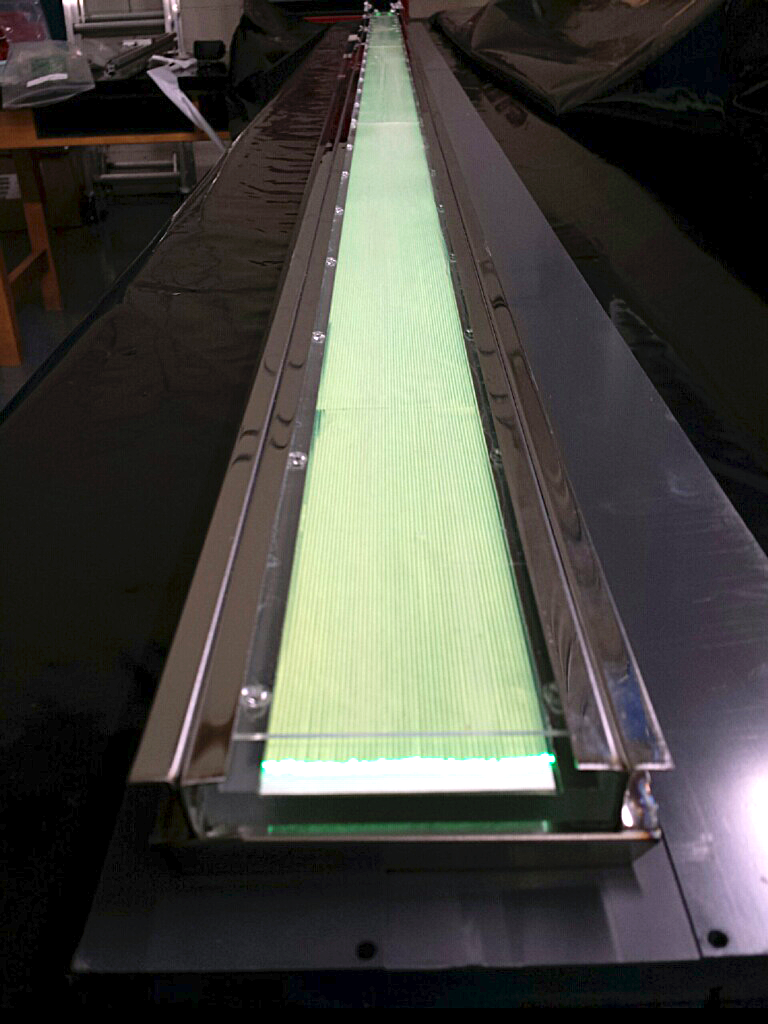
\includegraphics[width=.4\columnwidth]{fiber_bundle_1.png}
\end{cdrfigure}


The VUV photons are incident on the TPB-coated plastic radiator and
roughly half of the photons converted in the radiator are incident on
the %bundle 
fiber bundle. %The photons in the Y11 fiber 
These photons are then directed onto SiPMs at one end. The Y11 fiber (from Kuraray ) have
mean absorption and emission wavelengths of about 440~nm and 480~nm
respectively.  The attenuation length of the Y11 fibers is given to be
greater than 3.5~m at the mean emission wavelength, which allows
production of full-scale (2.2-m length) photon detector paddles.

First prototypes of this design utilized two rows of fibers with a
reflector behind the double row used to redirect the unabsorbed $\sim$400~nm photons back
through the two rows.% if they weren't absorbed on the first pass through. 
%Based on 
Data taken at the CSU Cryogenic Detector Development
Facility (CDDF) and the Fall 2014 FNAL Tallbo test 
showed that the front row of fibers collected
twice as much light as the back row, thus
only a single row
design can be considered --- this is currently under development. The current design
utilizes two single rows of fibers back-to-back with layers of \fixme{opaque?}\fixme{Carlos: no need to say opaque} Tyvek
diffuse reflector between them.

%Another benefit of this design is that an arrangement with back-to-back rows of fibers separated by an opaque relector arranged would then

In this design \fixme{what? the fiber bundles?} \fixme{Carlos: yes}would face into different TPC cells, allowing additional information to be
used in the disambiguation of the TPC signals coming from wire
wrapping on the APA frames. \fixme{signals coming from wire wrapping? How about `signals coming from wires on the APA frames'?}
If the walls of the detector were to be 
%A possible further benefit of the design could be its
%compatibility with concepts where the walls of the detector are
covered with TPB-coated material shifting the VUV photon to blue,
 the WS-fiber in this design could capture the emitted light, offering 
 a further benefit. Further study is
required to determine the effect these enhancements would have on the physics
reach of the detector. 

To fully exploit this approach several design optimizations need to be
be examined, including the following:

\begin{itemize}

\item{TPB coating thickness on thin radiator}

\item{Double-ended readout; if the fibers are read out from both
  ends and the corresponding channels are ganged onto one readout
  channel, an increase in channel output can be obtained without
  significant cost}

\item{Use of custom-doped fibers to best match the QE response of the
  SiPMs and the emission spectrum of the TPB}

\item{Removal of the radiator and coating the TPB directly onto the outer
  fiber-cladding of the Y11 fibers. Since the fibers are double-clad
  it may be the case that the attenuation lenth of the fibers is not
  altered by the TPB application. The geometry of the close-packed
  fiber row may lead to increased photon (400~nm) collection}

\end{itemize}

The cost of this design is comparable to that of the bar-based design
but is slightly more complex to fabricate --- although the Y11 fibers
are commercially available, which is an attractive feature. The
engineering aspects of the design will be discussed in the appropriate
section of this chapter. \fixme{ref section}

\section{Silicon Photomultipliers}

Silicon Photomultipliers (SiPMs) have been selected as the reference design  photon
detectors for the far detector LArTPC.% photon detection system. 
\fixme{Do we say `a sipm' or `sipm technology'? Plain `sipm' sounds funny.} \fixme{Carlos:yes,  it is standard terminology, right?} A SiPM is
a photo detection device sensitive to single photons with excellent
linearity range \fixme{`linearity range' means linearity over range of wavelengths? Plz clarify} in collecting multiple photons.  A SiPM consists of a
large avalanche photodiode (APD) array built on a common silicon
substrate. APDs operate in Geiger mode. \fixme{operates like a geiger counter?  I'd say, either give a more complete description of how they work or leave this off. Feels like it's out of the blue. Just MHO. AH} 

SiPMs have been developing at a very fast pace in recent years, in
response to the needs of the medical industry. As a result, the price of
SiPMs has gone down, while their performance has greatly
improved. A number of characteristics make SiPMs an
attractive choice as photon detectors for the PD system:

\begin{itemize}

\item{High photon-detection efficiency (PDE), up to 40-50\% at the
  peak detection wavelength. }

\item{High intrinsic gain ranging from 105 to 107 depending on the
  overvoltage}
\item{Low dark rate at cryogenic temperatures --- less than 50 Hz even
  at the maximum overvoltage}
\item{Insensitivity to external magnetic field}
\item{Extremely linear gain vs. overvoltage}
\item{Low cost per sensitive area compared to small cryogenic
  photomultiplier tubes (PMTs)}
\item{Small dimensions allowing a simple, compact and robust design}
\item{No need for high voltage (HV) power.}
\item{Low bias voltage, typically less than 100~V required, and even
  less than 30~V in some cases, resulting in low peripheral costs}
\item{Maintenance of high gain and PDE at cryogenic temperatures}

\end{itemize}

In short, SiPMs have demonstrated performance comparable to
traditional PMTs, but at a significantly reduced cost and %. As a result, they have become a 
are the photon-detector of choice for PD system of the far
LArTPC detector.

The main risk associated with using SiPMs is  %generally they have
%not been designed for 
operation at LAr temperature. %None of the 
SiPM
data sheets neither show nor guarantee the device's performance at cryogenic
temperatures. %This was the main motive for testing SiPMs at LAr temperatures. 
Most of the low-temperature tests performed by LBNE teams on SiPMs in the last two years have been
done using LN2, as it has similar temperature (10~K below LAr) but
costs much less.

A number of \fixme{remove the 1st SiPM simply manufacturers}SiPM manufacturers offer SiPMs, such as SenSL,
Hamamatsu, KETEK, AdvanSiD, CPTA (Photonique), Philipis, Novel Device
Laboratory (NDL), Zecotek, Voxtel, Amlification Technologies,
Excelites, %etc, 
but only a fraction of them offer SiPMs 
suitable for the PD system --- large area ($6\times6 mm^2$ or $3\times3 mm^2$), large fill
factor, pin or surface mount and no housing. An
exhaustive search of suitable SiPMs was conducted in 2012 and
sample SiPMs were obtained from SenSL, Hamamtsu, CPTA and
AdvanSID. It should be noted, however, that 
%although one should keep in mind, that in this rapidly developing field, manufacturers come up with 
new, improved models appear every year from most manufacturers.

%There are many SiPM suppliers on the market. \fixme{Carlos: this has been already said}
The initial round of
tests included models from SenSL (MicroSM-600-35-X13), Hamamtsu(MPPC
S10985-100C), CPTA (SSPM-0710G9MM) and AdvanSID (ASD-SiPM3S-P).
%, as we
%had success in obtaining suitable models from these four companies. 
In
this test, SiPMs were cooled in liquid nitrogen, laser light pulses at 400~nm
wavelength were used as the light source and signal output as a
function of overvoltage was recorded. Results can be seen in Figure~\ref{laser400}.

\begin{cdrfigure}[SiPM signals as function of bias voltage in liquid
    nitrogen.]{laser400}{SiPM signals as function of bias voltage in
    liquid nitrogen. Liquid nitrogen has 10 K lower temperature than
    liquid argon, making the measurement applicable. In all cases
    there is a significant increase in gain with increasing bias
    voltage, but difference in gain among different samples is clearly
    visible.} 
  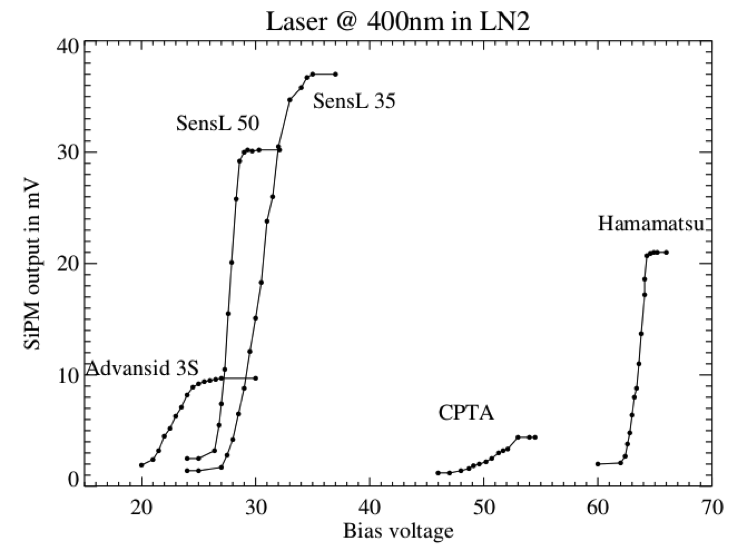
\includegraphics[width=.8\columnwidth]{sipm_laser.png}
\end{cdrfigure}

Based on these initial tests and high price
quotes received at the time from AdvanSiD and CPTA, the follow-up tests focused on SenSL and
Hamamatsu models. \fixme{but not the models already tested? Clarify (per the below)} % This decision was partially driven by .

Shortly after initial tests, SenSL came up with a new model
(MicroFB-600-35-SMT followed by improved MicroFC-600-35-SMT) and most
of the tests \fixme{so the `follow-up' tests were done on these new models?} have been done on the SenSL models. Hamamtsu’s MPPC
S12895- 0404-PB50 has been on the market for a long time and Indiana
group measured very high cross-talk and afterpulsing rates. \fixme{Do we need prev sentence?} Hamamtsu
%came up with 
released a new, improved model in 2015, S13360, that will be
tested in 2015 and compared with SenSL models.

\fixme{Can we summarize the current status? Which model is in the lead?}

\subsection{Requirements}

Despite argon's excellent scintillation yield, the PD system requires high-sensitivity photon detectors % to detect the scintillation light 
due to
the very small surface area of the SiPMs. %PDs.  
Furthermore, the late scintillation light in
argon reprsents 2/3 of the total, %scintillation light, 
but it is spread
over 1100 -- 1600~ns, making the individual late-light signals very
small on average.

%SiPM characteristics from the data sheets satisfy these requirements
%in general \fixme{be more specific than `in general'. I'm left feeling like
%you're not telling me something.}. Thus, 

SiPM data sheets indicate that these requirements are satisfied, but
it is important to observe similar performance
%is observed 
at LAr temperatures in terms of high gain, sensitivity to
single photoelectrons, high PDE, linearity of response, stability
of breakdown voltage, long-term stability, low afterpulsing and low
cross-talk. In addition, SiPMs must exhibit mechanical
robustness and low dark rate as they undergo cryogenic cooling and cycling. Finally, the cost must be low enough. To avoid sole-sourcing, it is required
%devices must have low cost and we need 
to identify at least two
choices that meet all the requirements. % to avoid sole source issues.

Institutions designing different PD prototypes (IU, CSU and LSU) %(Indiana University, Colorado State University and Louisiana State University)  you've already used the acronyms.
have
conducted a number of tests of PDs with SiPMs. \fixme{Make sure PD always refers to the whole thing not just the sipm} Additional,
specifically targeted tests have been conducted at LSU and University of Hawaii (UH) in recent
months. %The importance of selecting the best photo-sensors for the PD
%motivates the need for 
The parallel tests conducted at LSU and
UH will ensure important cross-checks and reduce
possible testing biases --- this is important for selecting the best photo-sensors.

\subsection{Test Results}

In the last 18 months, a test setup for SiPM evaluation has been built,
that includes Belle experiment \fixme{ref?} electronics to power and record signals
from SiPMs.  More recently \fixme{`in the last ...' might be very recent. ``In the last couple or few months?''}, a new board similar to the
SenSL testing board has been designed to address noise problems and low amplification
found on the Belle board, issues that become critical at low light levels. This new board is currently
being used to conduct dark rate and single-photoelectron studies.
Figure~\ref{sipm_schem} shows the layout of this board and a
picture of the actual circuit as built.

\begin{cdrfigure}[The schematics of the
    PCB board and the PCB as
    built]{sipm_schem}{The diagram on the left shows the schematics
    of the PCB board. The picture  on the right shows the PCB as
    built. This PCB can accommodate three SiPMs for testing.}  
  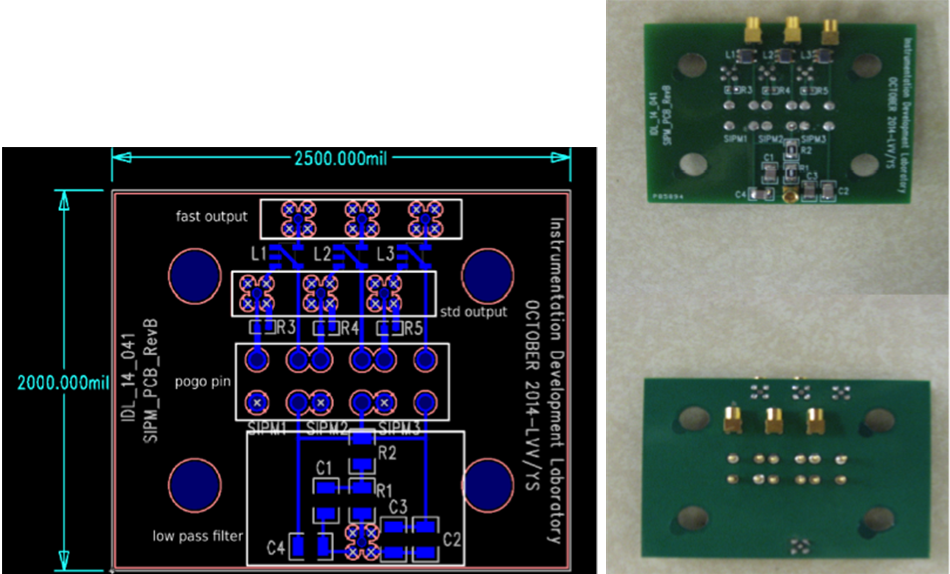
\includegraphics[width=.9\columnwidth]{pd_SiPM_schem.png}
\end{cdrfigure}

As previously mentioned, tests focused on Hamamatsu and SenSL produced
8 SiPMs.%\fixme{Carlos: tests focused on devices from Hamamatsu and SenSl} \fixme{tests produced a device? Plz clarify} However, the IU group found out that Hamamatsu
SiPMs are placed in a dewar inside a copper plated dark box and cooled
with LN2. SiPMs are held in place on the PCB with acrylic holder as
shown in the Fig~\ref{sipm_mount}. \fixme{This pgraph is confusing}

\begin{cdrfigure}[Acrylic holder for SiPMs and 
    assembly prior to lowering in the dewar]{sipm_mount}{Picture on the left shows acrylic holder that
    secures SiPMs to the PCB while figure on the top right shows the
    entire assembly prior to lowering in the dewer. Orange cable
    delivers laser or LED light that shines on the SiPMs. Everything
    is secured to the wooden lid that closes the dewar.}   
  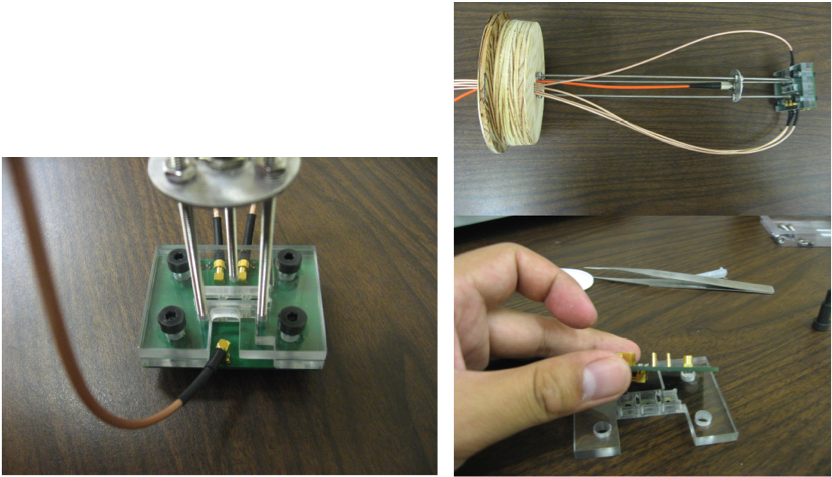
\includegraphics[width=.8\columnwidth]{sipm_mount.png}
\end{cdrfigure}

Different contraction rates of materials in
LN$_2$ produced mechanical damage to some of the SiPMs. To address this issue, a PCB board
with spring-loaded POGO pins is used (based on the previous design by
the CSU group) to provide contact to SiPMs and
hold them in place with acrylic housing rather than solder joints. Special cryo-rated, compact MMCX connectors have been acquired, as the
solder joints of the signal and power wires have been breaking from
repeated usage.

The SiPM bias voltage is delivered via the POGO pins and the SiPM signal is
sent via these pins to the DAQ. The signal is amplified via two inline
low-noise amplifiers and read out by oscilloscope. SiPMs are
illuminated by 1-ns-long laser pulses from the tunable wavelength
laser system. Laser light intensity is regulated with a Fine Laser
Intensity Controller (FLIC), a computer-controlled system that allows
tuning of laser intensity through several orders of magnitude with
various stages; this is important for linearity measurements. Signal waveforms
from a Waverunner LeCroy oscilloscope are recorded and analyzed.

It has also been noted that the SiPMs require lower bias voltage when
cooled in LN$_2$, which requires determination of the optimal operating
voltage at LAr temperature, since dark rates also increase with bias
voltage. Additional tests showed excellent gain at cryogenic
temperatures, as can be seen from the tests conducted on the SenSL C
series SiPM MicroFC-600-35-SMT (previous M and B series also tested) \fixme{do we need prev (...)?}
shown in Figure~\ref{sipm_gain}, along with clearly distinguished pulses
for one, two, three and four photelectron pulses.

\begin{cdrfigure}[Gain test of SenSL C series SiPM in LN$_2$ and 
    numbers of p.e.'s]{sipm_gain}{SiPM SenSL C series gain tested in LN2 is
    shown on the right hand side. Excellent linearity over the entire
    overvoltage range observed. There is a significant change of gain
    with increasing bias voltage, effectively doubling between the
    minimum and maximum tested bias voltage. Clearly distinguished
    numbers of photoelectrons can be seen in the left hand figure.}    
  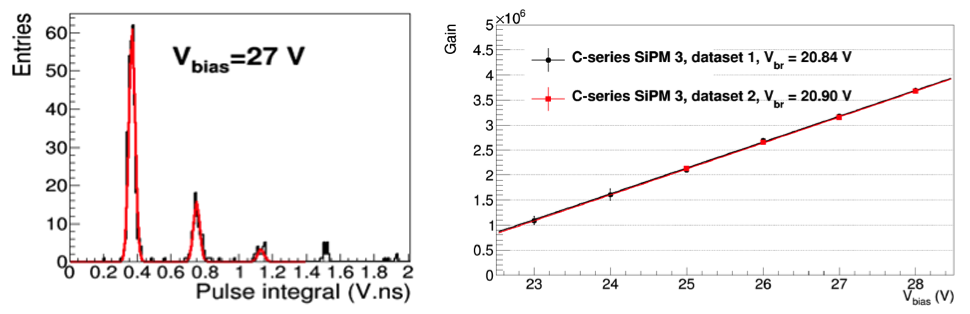
\includegraphics[width=1.0\columnwidth]{sipm_gains.png}
\end{cdrfigure}

The dark rate increases significantly with bias voltage, but the
overall rate is very small when SiPMs are cooled to 80~K, as can
be seen in Figure~\ref{sipm_dark}.

\begin{cdrfigure}[SiPM SenSL C series dark rate, two
    data runs in LN$_2$ ]{sipm_dark}{SiPM SenSL C series dark rate with
    two different data runs in LN2. While dark rate increases for an
    order of magnitude, it is still less than 50 Hz even at the
    highest bias voltage setting.}     
  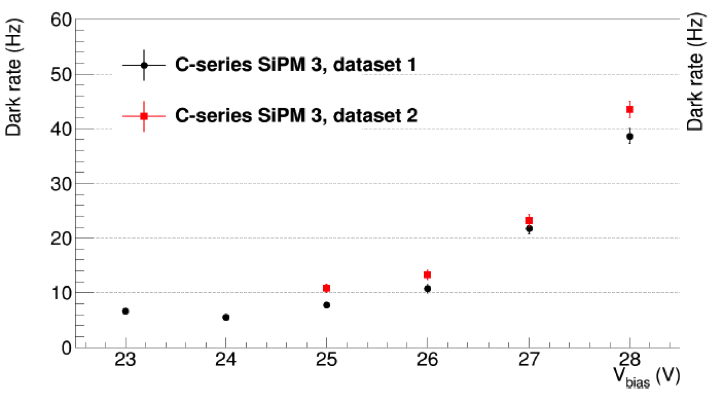
\includegraphics[width=0.8\columnwidth]{sipm_dark_rates.png}
\end{cdrfigure}

Afterpulsing is another important aspect of SiPM
performance. Afterpulsing increases noise and obstructs detection of
late argon scintillation light. Results of the afterpulsing
measurement performed on the cooled SenSL C series SiPM show a
very small afterpulsing fraction below 1\% for most overvoltage
values, as can be seen in Figure~\ref{sipm_after}.

\begin{cdrfigure}[SenSL C series SiPM afterpulsing fraction comparison, with system cooled]{sipm_after}{SenSL C series SiPM afterpulsing fraction for 5
    different SiPMs, with system being completely cooled down.}      
  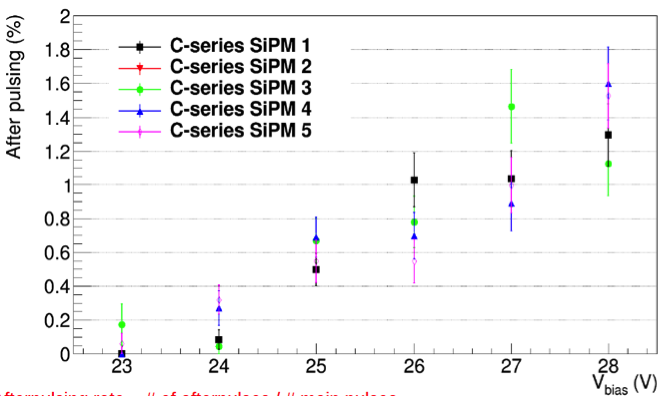
\includegraphics[width=0.6\columnwidth]{sipm_afterpulsing.png}
\end{cdrfigure}

SenSL C series SiPMs were also tested for cross-talk. Cross-talk gives
a measure of the light hitting one pixel \fixme{this seems wrong, plz check}, also produces signal in
adjacent pixels and effectively distorts the signal
strength. Figure~\ref{fig:sipm_crosstalk} shows the test
results. Cross-talk is a strong function of overvoltage, which will be
another criterion in choosing the operating overvoltage for the PD
system.

Although not presented here, SenSL B series SiPM MicroFB-600-35-SMT
were also tested and satisfy our requirements, based on the tests
conducted so far. However, we have not performed yet a full set of
tests including mechanical integrity from thermal cycling and
cross-checks. \fixme{Is this in the running? If not, leave out. If so, why not mentioned till now?}

\begin{cdrfigure}[SenSL C series SiPM cross-talk measurement based on
    two runs in LN$_2$]{sipm_crosstalk}{SenSL C series SiPM cross-talk measurement
    based on two separate runs in LN2. Cross-talk is a strong function
    of overvoltage and is very consistent between the runs.}       
  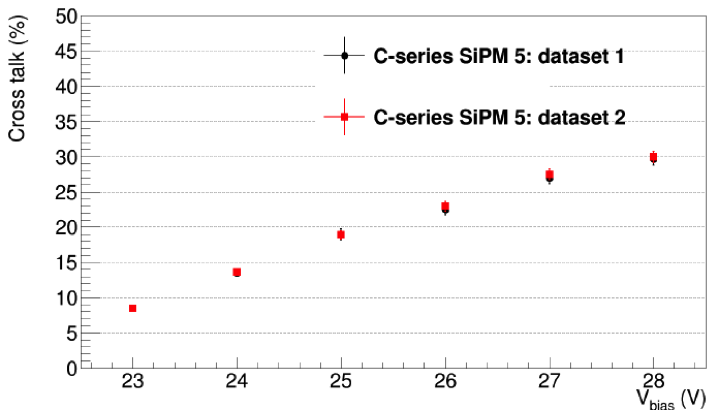
\includegraphics[width=0.6\columnwidth]{sipm_crosstalk.png}
\end{cdrfigure}

In parallel with performance tests, mechanical cryogenic tests are being
conducted where the number of cycles and time spent at LN$_2$ temperature
is being logged. This important test has started recently, but will
involve testing a number of devices for extended period of time and
examining their mechanical status under the microscope.% along with performance tests. 

Future steps involve increasing the testing sample of C series SiPMs
and evaluating several alternatives to avoid the risk of sole-source
vendor. 


\section{Mechanical Support}

Mechanically supporting the PD systems in the APA frames
presents several challenges, including the need to support three
different light-collecting and wavelength-shifting technologies in a
package utilizing the same mounting features in the APA frames, and
the effects of varying thermal contraction of various materials at 80
degrees Kelvin which complicated both light collector and SiPM
mounting. \fixme{devices of the 3 technologies are packaged together 
and the package is mounted on the apa? or the three all use the same
mounting features? I'm confused}

The baseline \fixme{reference?} design for mounting the PDs into the APA frames calls for
ten PD modules, approximately 2.2 m long, mounted with roughly equal
spacing along the full length of the APA frame (Figure~\ref{fig:5.5-1}).  The
PD modules are read out using individual twisted-pair cable, one per
SiPM.  These cables (120 of them in the original baseline \fixme{reference?} design) are
routed through the APA side tubes to a connector at the cold
electronics readout end of the APA.  Initially it was decided that it
would be too complicated to design the APA frames to allow PD module
installation following APA wire-wrapping, so it was planned to install 
the PD modules %were installed 
prior to this step.% in the installation process.  
The
wavelength-shifting elements in the light collectors of the PD modules
are sensitive to heat, humidity and most critically to %exposure to
ambient light, which places significant requirements \fixme{constraints?} on the
environment in which the APAs are assembled and stored,% in this way, 
%but initially it was decided this was the best option.
\fixme{Something about how this is still better than installing them after wire-wrapping; list a risk or two of that method, maybe, for comparison}

\begin{cdrfigure}[Full APA frame with ten photon detectors mounted
  inside the frame]{5.5-1}{Full APA frame with ten photon detectors mounted
  inside the frame}
   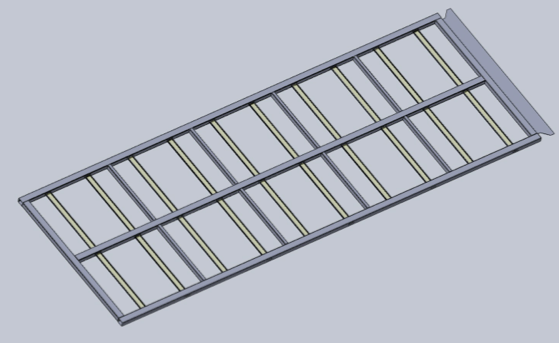
\includegraphics[width=.6\columnwidth]{fig5-5-1.png}
\end{cdrfigure}

A universal PD frame assembly was devised to hold all three PD design
variations under consideration.  Figure~\ref{fig:5.5-2} shows an example of a
short (400-mm-long active area) version of this frame manufactured for
the 35t test, \fixme{figure could use labeling} and Figure~\ref{fig:5.5-3} shows a mechanical assembly drawing of
the frame system for one of the candidate light collector choices.
The frame consists of two plastic (acetal) end caps mounted to the
inside of the APA frame, joined by 10-mm-diameter stainless steel tubes
that run the full width of the APA frame, providing intermediate
support for the PD modules.% as needed.  
The SiPM mount PCBs \fixme{I can't parse this phrase} are
incorporated into one of the end blocks, along with the cable
connections for the twisted-pair cables.  Due to the significant
%variations in 
difference between the coefficients of thermal expansion for the stainless
steel frame and the plastic WLS elements, %we expect 
a relative
difference in thermal contraction of $\sim$1\% is expected at LAr temperatures.  The
far endblock assembly provides balancing forces to the light collector
elements %as required 
to ensure these elements remain %in 
straight and
in good contact with the SiPMs.

\begin{cdrfigure}[Photograph of 40~cm long bar-based prototype mounted in test frame]{5.5-2}{Photograph of 40~cm long bar-based prototype mounted in test frame}
  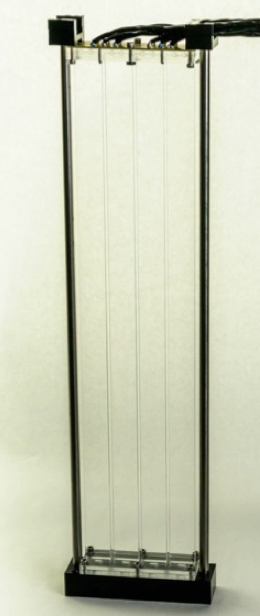
\includegraphics[width=.5\textwidth]{fig5-5-2.png}
\end{cdrfigure}


\begin{cdrfigure}[Mechanical assembly drawing of frame system]{5.5-3}{Mechanical assembly drawing of frame system}
  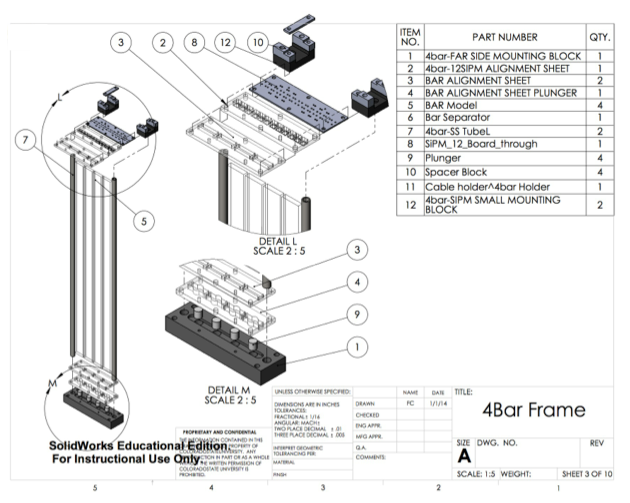
\includegraphics[width=\columnwidth]{fig5-5-3.png}
\end{cdrfigure}


Testing of the PD mount scheme in many test setups (at IU, CSU and
FNAL), as well as experience APA assembly, have led to a re-evaluation
of the PD mounting scheme.  The revised baseline \fixme{} has PD installation
%occurring following 
after APA wire wrapping, through slots left in the side
of the APA frame (Figure~\ref{fig:5.5-4}).  As shown in the figure, the
plan still calls for ten PDs per APA frame.  Five of the PDs will be
installed through each side of the APA frame, and the cables for each
of the PDs will be routed to the cold-electronics end of the APA,
inside the side tube through which the PD was inserted.  Stainless steel
c-channels mounted into the APA frames prior to wire wrapping will
guide and support the PDs during and after installation.  The PD will
only be attached to the APA frame at one end, so the purely plastic PD
module will be free to slide in the track to allow for the
differential contraction (Figure~\ref{fig:5.5-5}).  Tests of the 2.2-m prototype
assemblies of both fiber hybrid and the LSU-proposed monolithic
acrylic bar design in the CSU CDDF \fixme{what's cddf?} have demonstrated significant
promise.  %This installation scheme

\begin{cdrfigure}[Blow up of APA fram showing PD insertion location]{5.5-4}{Blow up of APA fram showing PD insertion location}
  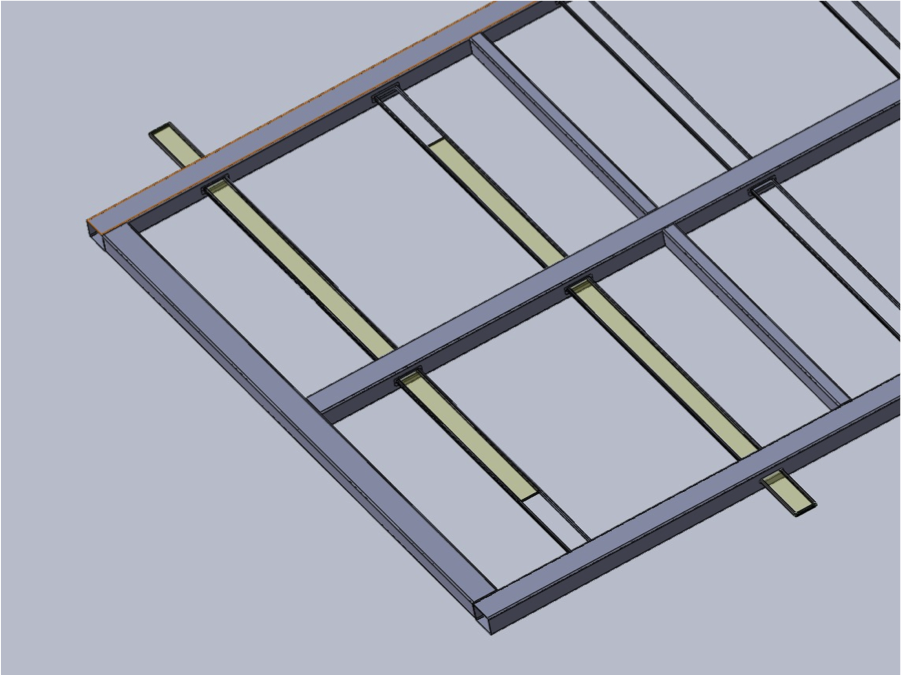
\includegraphics[width=.6\columnwidth]{fig5-5-4.png}
\end{cdrfigure}


\begin{cdrfigure}[Slot and rail showing mounting location of photon detector]{5.5-5}{Slot and rail showing mounting location of photon detector}
  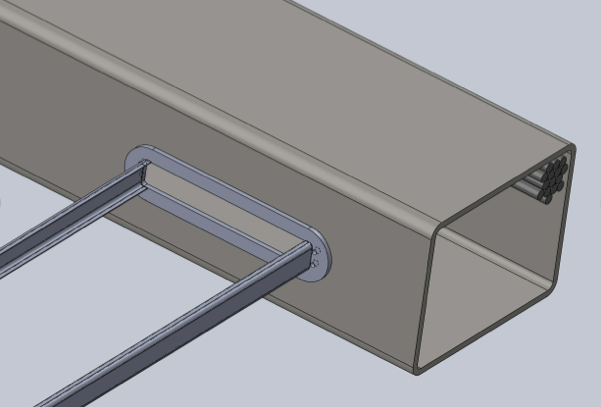
\includegraphics[width=.6\columnwidth]{fig5-5-5.png}
\end{cdrfigure}


Thermal contraction at cryogenic temperatures also complicates the
mounting of the SiPMs in the PD modules.  The baseline \fixme{} sensL SiPMs are
surface-mount components, with four $0.5\times0.5$-mm pads for making
electrical contact.  Unreliability \fixme{?} and elevated dark count rate
problems, as well as physical delamination of the SiPM front face from
the silicone substrate, were observed early in cryogenic testing of
SiPMs, and suspicion fell on the mechanical contact between the
mounting PCB and the SiPM itself.

Three different methods of making these electrical contacts have been tested\fixme{?}: 
\begin{itemize}
\item Soldering
the SiPMs directly to the PCBs (fig 5.5-6a), 
\item using commercial
spring-loaded electrical contacts or ``Pogo pins'' (Figure~\ref{fig:5.5-6b}),\fixme{check ref} 
\item soldering short wires to the SiPM pads and thence to the PCB
(Figure~\ref{fig:5.5-6c}).\fixme{check ref}  
\end{itemize}
Each of these methods provides assembly challenges,
and cryogenic testing has not suggested a clear choice so far.
Testing and development are still underway to resolve this issue.

\section{Photon System Readout Electronics}
\label{sec_elec}

\subsection{Reference Design} %Added by AH to avoid single subsec for Alternatives'

Scintillation light from LAr comes from the two different excited
states \fixme{of Ar atoms?} with lifetimes of about 6~ns and 1.6~$\mu$s.  Only a limited
amount of light \fixme{can you be a bit more specific?} is collected by the PD system, so the electronics must
be designed to collect the light from both excited states. A summary
of the general requirements for the system, including requirements
from a physics performance perspective, are given in
Table~\ref{tab:fee_req}.
%
\begin{cdrtable}[Physics requirements for the photon detector electronics]{ll}{fee_req}
{Physics requirements for the photon detector electronics}
 Performance Parameter       & Target   \\ \toprowrule
 Time Resolution                   & Better than 30 nS wrt event time zero ("t0")       \\ \colhline
 Charge Resolution               & 0.25\% photo-electron equivalent                      \\ \colhline
 Dynamic Range                   & $\sim \times$10 better than detector (1000:1)          \\ \colhline
 Linearity                               & Sufficient to resolve 1 photo-electron signals   \\ \colhline
 Multi-Hit Capability              & Sufficient to measure Triplet (late) Photons           \\ \colhline
 Dead Time                           & Live up to 2 drift times either side of beam spill           \\ \colhline
 Bias Control                        & 0.1 V resolution up to 30 V per channel   \\ \colhline
 Calibration                          & On-board Charge Injection   \\ \colhline
 Timing                                 & Events time-stamped using NO$\nu$A Timing syst.  \\
\end{cdrtable}


%
The plans for the electronics for the photon detection subsystem
include a baseline \fixme{} design with several options that remain R\&D
activities.  There alternative implementations of electronics are
described in Section~\ref{sec_alt}.
%These options are identified in the description that follows.  
%There are also some alternative implementations of electronics that remain under consideration.  These are described in Section~\ref{sec_alt}
%These are described in Section 6.4.

In the baseline \fixme{} plan, there are no front-end electronics in the cold
volume.  Instead, the unamplified signals from the SiPMs are
transmitted to outside the cryostat on cables for processing and
digitization, as shown in Figure~\ref{fig:fig-e-1}.  There are
advantages and disadvantages to this approach.  The advantages are
that the infrastructure required for inside the cryostat is reduced
(power, data cables, precision clocks, data protocols, etc.);
reliability is improved (no single-point failures of multi-channel
devices inside the cryostat); serviceability and accessibility to the
front-end electronics are improved; and the need to develop cold
electronics, possibly a custom ASIC, is eliminated.  The disadvantages
are that the cable plant inside the detector is increased, which can
create mechanical challenges and installation difficulties; the flange
board (warm/cold interface) is more complex; there are generally more
connectors in the system; and signal-to-noise considerations are more
difficult.  %Generally, t
The baseline  \fixme{} design favors simplicity,
reliability and reduced R\&D time and costs, and also meets the
performance requirements of the electronics.
%
\fixme{No fig1 exists for: Block diagram of the photon detector signal processing system.  }
%
\begin{cdrfigure}[Block diagram of the photon detector signal processing system]{fig-e-1}{Block diagram of the photon detector signal processing system}
%\includegraphics[angle=0,width=10cm,height=7cm]{fig1}
\end{cdrfigure}

In the 35t prototype, each SiPM signal was \fixme{not `is'?} transmitted on an
individual shielded twisted-pair cable fitted with individual
LEMO-style connectors.  The bias voltage was coupled onto the signal
cable, using AC-coupling on the receiving end to measure the SiPM
signal.  The use of high-quality cable with point-to-point connections
between an individual SiPM inside the cryostat and the front-end
electronics residing outside the cryostat, combined with good
differential signal processing on the receiving end, enabled the
demonstration of the principle that single photo-electron signals
could be measured accurately without the need for cold electronics.
In order to address the problems with the cable plant as identified
above, the following ideas are being pursued:
\begin{itemize}
\item Ganging together several SiPM outputs from a given PD
  detector into one output cable.  This increases the detector
  capacitance, affects the pulse shape, and could spoil the timing
  resolution of the measurement.  Also, the SiPMs may have to be
  preselected, since there will be only one bias voltage for three
  devices, and it may be important to match the overvoltage
  characteristics.  Studies are in progress to find a compromise
  between data precision and cabling issues. One approach is to add a
  cold pre-amplifier if the ganging together of several SiPMs result
  in performance that is too degraded to meet specifications.  The
  infrastructure requirements (cables, connectors, power, cold
  performance, reliability, mechanical mounting, etc.) would have to
  be considered.

\item Use of multi-conductor, individually shielded pair \fixme{if it's a pair, is it just dual-conductor? This is confusing} cable.  A
  candidate cable containing four individually shielded twisted pairs
  has been identified and tests are in progress.  The cable is in
  Teflon jacket, which should be \fixme{has been found to be?} acceptable for use in LAr.

\item Use of mass-terminated connectors.  Several candidate connectors
  for use with the cable described above are being pursued.
\end{itemize}

The baseline  \fixme{} plan assumes that three SiPM signals \fixme{outputs?} can be ganged
together into one readout channel.  By using the multi-conductor cable
with four twisted pairs, this results in one cable per PD consisting
of 12 SiPMs.  The diameter of this cable is ~xxx-mm, \fixme{get number} which reduces the
cable plant by $\sim \times$10 compared to that used in the 35t
detector.  The cost of the connectors also decreases by $\sim \times$10.
Lastly, the ease in making connections at the flange board will be
improved by the use of a mass-terminated connector.

In the baseline\fixme{}  plan, the front-end electronics reside outside of the
cryostat in instrumentation racks.   A
custom module for receiving SiPM signals has been designed and built, and signal
processing is being performed in the front-end as preprocessing for trigger and DAQ.  The
module is called the SiPM Signal Processor (SSP).  An SSP consists of
12 readout channels packaged in a self-contained 1U module.  Each
channel contains a fully differential voltage amplifier and a 14-bit,
150~MSPS analog-to-digital converter (ADC) that digitizes the
waveforms received from the SiPMs.  The front-end amplifier is
configured as fully differential with high common-mode rejection, and
receives the SiPM signals into a termination resistor that matches the
characteristic impedance of the signal cable.  Currently there is no
shaping of the signal, since the SiPM response is slow enough relative
to the speed of the digitization to obtain several digitized samples
of the leading edge of the pulse for the determination of signal
timing.

The digitized data is stored in pipelines in the SSP for up to $\sim$
13~$\mu$s.  The processing is pipelined, and performed by a Xilinx
Artix-7 Field-Programmable Gate Array (FPGA).  The FPGA implements an
independent Data Processor (DP) for each channel.  The processing
incorporates a leading-edge discriminator for detecting events and a
constant fraction discriminator (CFD) for sub-clock timing resolution.
Because the FPGA is programmable and accessible, it is possible to
explore different data processing algorithms and techniques, and even
customize the readout for a given type of event (e.g., supernova).  A picture of the module is shown in Figure~\ref{fig:fig-e-2}.
A block diagram of the system is shown in Figure~\ref{fig:fig-e-3}.

%Figure xx3.  Picture of the SSP module.
\begin{cdrfigure}[Picture of the SSP module]{fig-e-2}{Picture of the SSP module}
%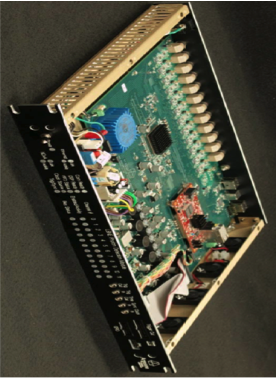
\includegraphics[angle=90,width=10cm,height=5cm]{fig-e-2.png}
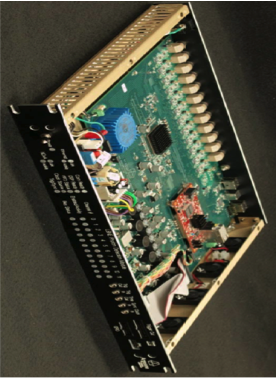
\includegraphics[angle=90,width=.9\textwidth]{fig-e-2.png}
\end{cdrfigure}

%Figure xx2.  Block diagram of the SSP.
\begin{cdrfigure}[Block diagram the SSP module]{fig-e-3}{Block diagram the SSP module}
%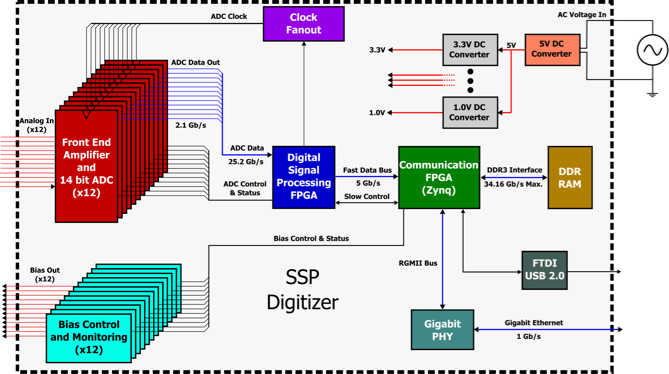
\includegraphics[angle=0,width=12cm,height=7cm]{fig-e-3.png}
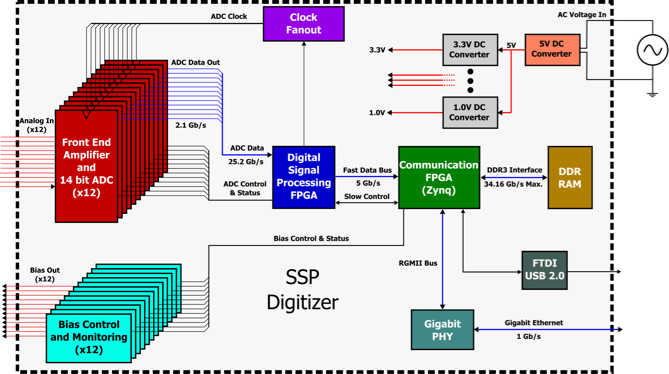
\includegraphics[angle=0,width=.95\textwidth]{fig-e-3.png}
\end{cdrfigure}

In the simplest mode of operation, the module can perform waveform
capture, using either an internal trigger or an external trigger.  Up
to 2046 waveform samples may be read out for each event.  When
waveform readouts overlap, the device can be configured to offset,
truncate or completely suppress the overlapping waveform.  Pile-up
events can also be suppressed.

As an alternative to reading full waveforms, the DP can be configured
to perform a wide variety of data processing algorithms, e.g., measuring amplitude (via several techniques), and %also 
timing the
event with respect to a reference clock.  All timing and amplitude
values are reported in a compact event record.  Each data processing
channel stores up to 340 event records when not storing waveforms. 

Generally,\fixme{There's that `generally' again!} the SSP performs pipelined processing.  The module has been
designed to support several different triggering schemes, including
self-triggering, use of an external trigger, or use of an external gate to
read out all events within a time window.  In order for the events
measured in the photon detector to be matched up with the
corresponding events in the TPC, the front-end electronics attaches a
timestamp to the data as it is acquired.  The timestamp is unique, and
has a correspondence with the timestamps in the TPC electronics
processing.  The timestamp in the SSP is applied to the event data as
it is digitized, and becomes part of the data as the processing
proceeds.  In the case where zero-suppression and data sparsification
are used, the timestamp on accepted data remains intact.  To achieve
this, the TPC and PD electronics must be synchronized, including
timestamp counter resets, and a known and stable calibration between
the corresponding timing resolution of the ADC conversion in the two
systems \fixme{not full sentence}.  The electronics has been designed to support a full
interface to the NO$\nu$A timing system, which is the baseline \fixme{} timing
system for the experimental prototypes.

A Xilinx Zynq FPGA, onboard %the 
a MicroZed system-on-module, \fixme{`the' makes it sound like we've heard of the microzed thing, but we haven't yet} handles the
slow control and event data transfer.  The SSP has two parallel
communication interfaces, USB 2.0 and 10/100/1000 Ethernet.  The 
1-Gb/s Ethernet supports full TCP/IP protocol.  The module includes a
separate 12-bit high-voltage DAC for each channel to provide up to 
30~V of bias to each SiPM.  The module also features charge injection for
performing diagnostics and linearity monitoring, and also voltage
monitoring. \fixme{``The module also features charge injection for
performing diagnostics, linearity monitoring and voltage
monitoring. `' or ``The module also features charge injection for
performing diagnostics and linearity monitoring, and it also features voltage monitoring. `'?}

In tests to date, the SSP is capable of measuring single
photo-electron signals coming from the SiPMs over a cable length of 30~m when the SiPMs are operated at LAr temperature.  The timing
resolution of the signals has been measured to be better than 3~ns.
The full-differential signal processing in the front-end circuitry is
important in achieving this result.
 
The SSP is self-contained in that it receives 60-Hz, 120-V power, and
has internal linear and DC/DC power supplies for generating the DC
voltages needed for the instrumentation %, as well as 
and the bias voltage
for the SiPMs.  The SSP is packaged in a 1U, rack-mountable
package. For the 35t prototype, the racks are located near the
ports on the top of the cryostat.

\subsection{Alternatives}
\label{sec_alt}

\fixme{Start with a sentence that says what alternatives this section discusses: CE, pulse-shaping, ASIC...  }

%%%%%%%%%%% CE

In the baseline \fixme{} design of the PD electronics, %the approach was taken to have 
no electronics are placed inside of the cold volume.  This results in a
large number of cables and connectors.  Other experiments using liquid
argon have successfully implemented cold TPC electronics, thereby
significantly reducing the cable plant that must come through the
cryostat.  

%This approach 
Using cold electronics \fixme{check} has challenges in power distribution, heat
dissipation, and the performance of front-end electronics in LAr. To
address serviceability, the cold electronics might be realized in a
modular way and situated just below the flange in the cryostat so that
it can be accessed for repair if needed.  To this end
the zero suppression will be important to avoid high data rates
depending on the number of readout channels needed. \fixme{prev sentence unclear. what depends on no. of channels?} %A way to realize
The cold zero suppression %would be to 
could be implemented by means of a cold FPGA (or an
ASIC, yet to be developed).  To date the cold FPGAs have had mixed
results in tests. 

%An alternative approach would be to perform an ``analog
%zero suppression'' with a constant-fraction discriminator and then gate
%the signal and digitize warm, in which case the complication with
%encoding the particular channel has to be addressed.  

%%%%%%%%%%% % analog zero suppression option

Performing an ``analog zero suppression'' with a constant-fraction discriminator 
provides an alternative approach; it would be followed by gating
the signal and performing warm digitization. This technique would, however, introduce the complication of encoding the particular channel. \fixme{I'm not sure I got this right; I didn't completely understand the orig sentence to begin with} 
%
The significant
challenges in this technique include power dissipation, the increased
possibility of contamination of the LAr, and extended infrastructure
%requirements 
that must reside in the cold volume.  %The virtue is that this 
On the other hand, it can significantly reduce the number of signal penetrations into
the cold volume.

%%%%%%%%%%%%  Pulse-shaping option

The electronics for the photon detector of LBNE uses fast (direct)
digitization of the SiPM pulses. Another option for the front-end
electronics is to use pulse shaping. Instead of digitizing the full
bandwidth of the SiPM signal, in this technique the pulse is shaped using analog
filtering techniques, generally producing a pulse with a prescribed
shape for which the peak is proportional to the total amount of charge.
By measuring the peak, both amplitude and pulse timing can be
obtained.  Since the pulse response follows a known transfer function,
the pulse peak can be obtained using slower synchronous sampling, or
using asynchronous sampling through the use of peak detection and
constant fraction discrimination.  

In either case, the data can be
processed by an FPGA using algorithms optimized for the application.
In particular, assuming that a sufficient number of samples of the shaped pulse are
obtained, a chi-square comparison of the shape to
the ideal pulse shape can be used to 
identify events or determine pulse corruption %, or event identification.  As with direct digitization, the digitization clock
\fixme{check}
and a timestamp can be synchronized using an external clock source. The
data can be read out in a similar manner, using USB 2.0 or 10/100/1000
Ethernet.  The virtue of this approach is that a slower ADC can be
used, reducing power consumption, data load and the
speed of readout links. \fixme{reducing speed of readout links is a virtue?} The technique trades bandwidth for
shaping, making timing and pile-up issues more important.  This can
result in making the interpretation of the pulse shape more complex, 
requiring more 
than direct digitization.  Generally, the pulse-shaping circuitry is
also less expensive than the direct digitization technique, assuming
similar performance requirements.

%%%%%%%%%%%%  ASIC option
Another option for the photon system readout would include the use 
of an Application Specific Integrated circuit (ASIC) as a way to
reduce cost.  The large channel count in a real detector system is
such that the production cost of the system could be greatly reduced. \fixme{how does large channel count relate to reduction in cost? }
Often, the cost of development of an ASIC from scratch is quite high,
of order $\sim$400K\$, and can take $\sim$1 to 2 years for development, so cost
and schedule must be weighed carefully.  However, other benefits from
the ASIC approach include reduced space requirements for circuitry on
the front-end, lower power dissipation, and specialized functionality
in the front-end chip.  

Several ASICs have been
designed over the last few years %especially 
for SiPM readout.  %One could potentially 
It would be possible to explore the functionality and performance of these
designs, for either for warm or cold electronics, and evaluate their suitability for LBNE.  %This option might be used either for warm or cold electronics.  
Direct digitization has
the virtue of being straight-forward from a circuit design
perspective.\fixme{connect direct digitization with ASIC}  By taking advantage of modern high-bandwidth OP amps,
high-speed, high-rate ADCs, and powerful FPGAs with high-speed serial
links, it is possible to obtain 14-bit dynamic range digitization with
$\sim$1-ns timing resolution.  By reading all of the samples into an
FPGA having a deep buffer, digital signal processing techniques can be
employed using the programmable logic; this could make it possible
to develop powerful analysis
algorithms %that can be developed 
in time.  The technique generally has
higher power consumption and tends to be more expensive than simpler
instrumentation techniques.

\section{Photon Detector Calibration}
\label{sec_pd_calib}

The photon detector calibration is a part of a larger calibration plan
that covers all aspects of a LArTPC detector calibration. The larger plan
 includes
methods to convert collected charge to initial particle energy, as
well as calibration techniques to convert collected scintillation
light into an estimate of a particle's interaction time, energy and a
track/vertex location for each event.  

As already described, the
baseline \fixme{} for the scintillation photon detectors assumes employment of
acrylic light collection paddles to reduce the required costly
photo-cathode area. Several photon detector designs are presently
being developed and are being tested in small dewars. Since %each 
none of
these new elements has %not 
yet been tested in a large-scale TPC, the
35t LArTPC prototype is being constructed to provide essential
design validation. 

The current FD designs are anticipated to have
sufficient sensitivity to provide event timing information for
atmospheric neutrino and proton decay channels. However, it will not
provide high efficiency down to the 5-MeV neutrino energy level
desired by the supernova program. %This would have the impact that the
This would cause the supernova event reconstruction energy resolution to be 20\% compared to the 5\%
achievable with %the event time determination from 
a photon detector
able to operate efficiently at a sufficiently low energy
threshold. The improvement in physics will be studied in the near
future but a substantial effort in development of improved detection
techniques is desired. 

In the absence of precise physics requirements
for the photon detector system and in order to support R\&D activities
on the photon detector development it was decided that the photon
detector should provide a time stamp to determine the time of
occurrence of an event (so called ``time zero'') with an accuracy much
better than 1~s \fixme{fix}.  

Items relevant to the photon detector calibration
are the fast and slow components of the light, photon propagation
including scattering and reflections, impact of N2, \fixme{what's N2?} E-field strength,
and the energy range of interest. A calibration system that
addresses the issues listed above has to be both comprehensive and
cost-effective, and has to be tied to the overall calibration system
that includes both charge and scintillation-light calibration
techniques. Such a system will be designed in the future.  \fixme{`is planned...'?}

To support
the PD R\&D phase a light-flasher-based calibration system
has been designed
that will serve to monitor the relative performance and time
resolution of the system. In particular, for the anticipated 35t
performance tests the relative efficiencies of
multiple light collection techniques must be evaluated in order to 
%be able to
down-select an optimal light-readout technology. The system that meets
these requirements will consist of a set of LEDs as light sources or a
laser with a VUV wavelength coupled to quartz fibers, thus
transmitting light from outside the detector volume to desired
locations at the CPA within a TPC. Therefore the 35t
detector will be equipped with LEDs located and fired externally, with fibers running
into the cryostat to diffusers that will emit light from the CPA to
the APA. 

%For the 35t cryostat at the surface at Fermilab it will be
%complementary to cosmic ray muon tracks as means of calibration. 
For the 35t cryostat, installed at the surface at Fermilab,  a light-flasher-based calibration system will be
complementary to calibration by cosmic-ray muon tracks.

%In terms of light sources t
The \fixme{35t calibration?} measurements should be performed with an UV
(245-375nm) light source. The UV light mimics physics starting from
the wavelength shifter conversion, through the light guide propagation,
photo-sensor detection and FEE readout.  The external light-flasher
calibration system is designed such that it:
\begin{itemize}
\item is simple to implement (has no active components within PD/APA, such as
  LEDs or fibers mounted within APA).
\item is less-intrusive (less fiber material is within detector %in terms of fibers 
than if each PD frame were equipped with individual fiber).
  \item
  provides a benchmark light-based reconstruction with the use of
  localized light sources distributed throughout the detector volume.
\item has the potential to be adapted for deployment in a large far
  detector% in the future
\end{itemize}

Figure~\ref{fig:fig-c-1} illustrates the system. It
consists of a 1U rack mount Photon Detector Calibration Module (PDCM)
sitting outside the cryostat. The module generates light
pulses that propagate through a quartz fiber-optic cable to diffusers
at cathode-plane (CPA) to distribute the light uniformly across the
photon detectors mounted within an anode plane (APA).  There are five
diffusers on the CPA plane: one in the center and four close
to the CPA corners, as shown in Figure~\ref{fig:fig-c-2}. 

%
\begin{cdrfigure}[Concept of the UV-light calibration system]{fig-c-1}{Concept of the UV-light calibration system for the photon
  detector in liquid argon} 
  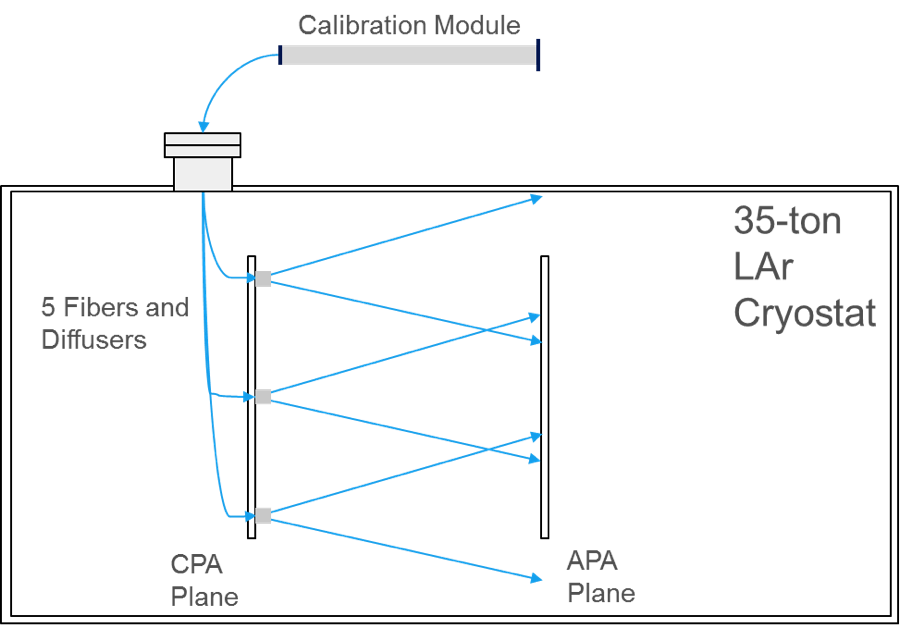
\includegraphics[angle=0,width=10cm,height=7cm]{fig-c-1.png}
\end{cdrfigure}


\begin{cdrfigure}[Diagrams of diffusers, their locations and UV light transport]{fig-c-2}{The diffuse light is emitted from diffusers (top left figure)
  mounted at five CPA locations, indicated by arrows (right figure).
  The UV light from the PDCM to diffusers is transported through
  quartz fiber (lower left figure).}
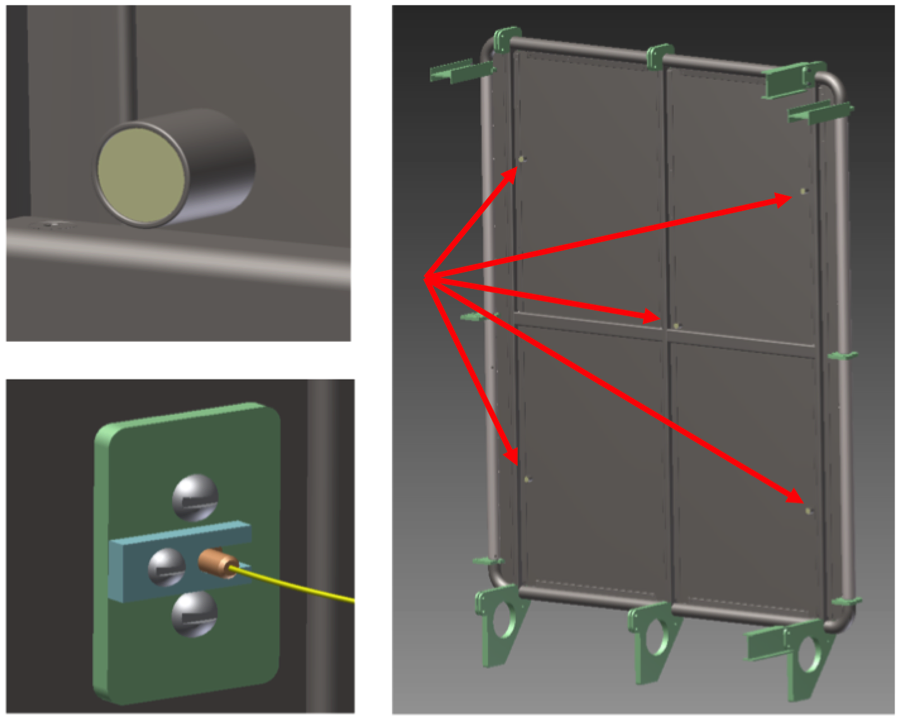
\includegraphics[angle=0,width=10cm,height=7cm]{fig-c-2.png}
\end{cdrfigure}


The PDCM module layout is shown in Figure~\ref{fig:fig-c-3}. The ANL
photon calibration module is based on a repurposed SSP unit.  An SSP
board will be repackaged into a deeper rack mount chassis that will
accommodate a new internal LED Pulser Module (LPM) and an additional
bulk power supply. The LPM utilizes five digital outputs to control
the LPM pulse and its duration (arrows in black).  These LVDS outputs
are derived from the charge injection control logic within the SSP's
FPGA.  The even-channel SiPM bias DACs are repurposed to control the
LPM pulse amplitude (arrows in red).  The adjacent odd channels are
used to read out a photodiode that is used for pulse-by-pulse
monitoring of the LED light output.  The output of the monitoring
diode is used to normalize the response of the SiPMs in the detector
to the calibration pulse

\begin{cdrfigure}[Photon detector calibration module (PDCM) layout]{fig-c-3}{Photon detector calibration module (PDCM) layout}
%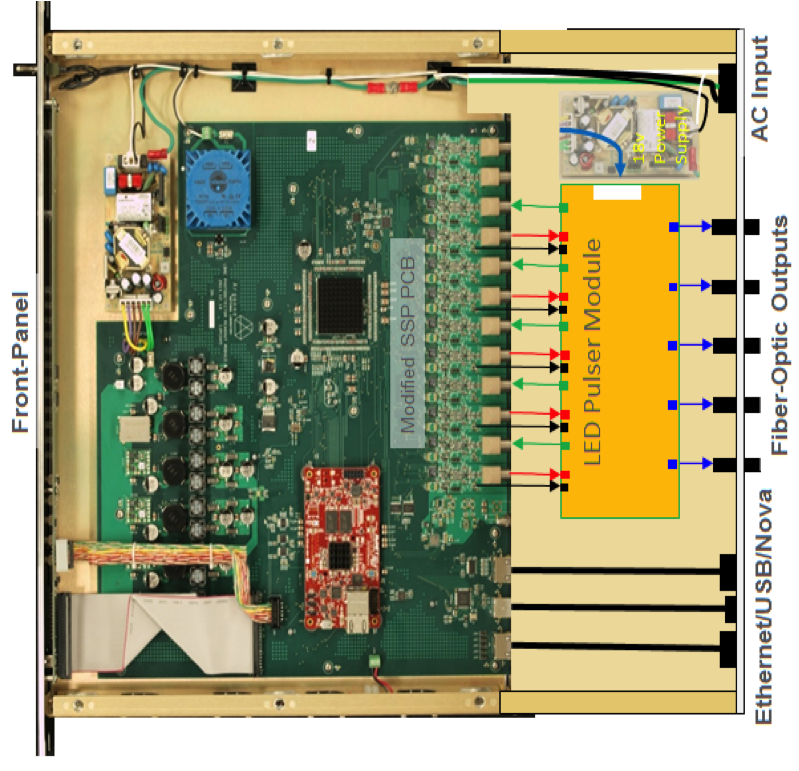
\includegraphics[angle=0,width=10cm,height=7cm]{fig-c-3.png}
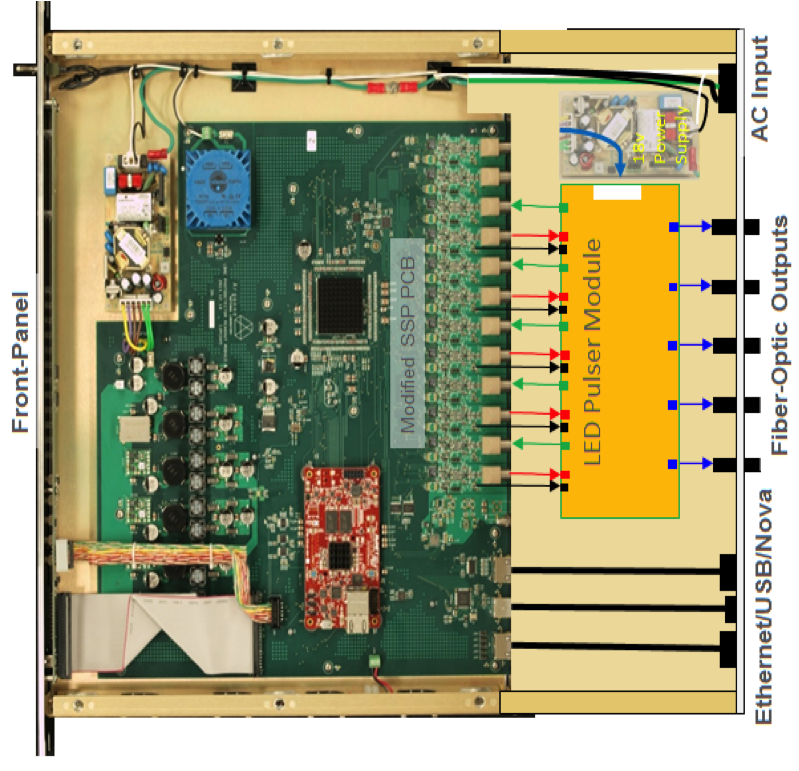
\includegraphics[angle=0,width=.8\textwidth]{fig-c-3.png}
\end{cdrfigure}


%For the 280~nm light we have performed a simulation of 
The designed
diffuse-light calibration system has been performed with 280-nm light using TracePro, a generalized 3D
light ray-tracing program with the ability to include bulk optical
properties such as absorption, fluorescence and birefringence in addition
to surface properties such as scattering and
reflection. Figure~\ref{fig:fig-c-4} shows simulated light distributions
of the 35t APA for the cases of the VUV light emitted by either
the central diffuser only (left figure), or by the outer four diffusers
simultaneously (right figure). A full Geant4-based simulation of the
detector will be used in the future. Using the preliminary data with
the 35t-style light guides (indicating 0.5\% efficiency for number
of photo-electrons per incident 128-nm LAr scintillation photon 50~cm
from the light guide), we estimate for 280-nm light to observe $\sim$15
photo-electrons per single SiPM channel when the light is emitted from
the single central diffuser in 13-ns-long pulses. Similarly, we expect
$\sim$100 photo-electrons observed by a single SiPM channel when 280-nm light is emitted in 100-ns-long pulses from the four outer
diffusers at once.

%
\begin{cdrfigure}[Simulated light distributions of the 35t APA, two cases]{fig-c-4}{Simulated light distributions of the 35t APA for the cases of the VUV light emitted by either the central diffuser only
  (left), or by outer four diffusers simultaneously (right).}
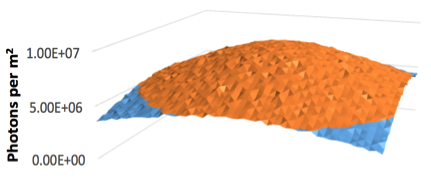
\includegraphics[angle=0,width=6.5cm,height=3.5cm]{fig-c-4-L.png}
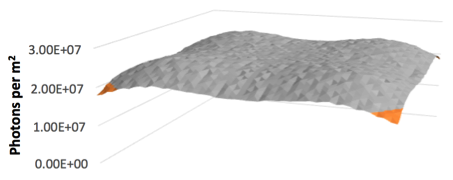
\includegraphics[angle=0,width=6.5cm,height=3.5cm]{fig-c-4-R.png}
\end{cdrfigure}


In the LBNE prototypes (i.e., the 35t) and in %Future 
the far detector it
will be important to check that photon-detector components are
functioning properly at various stages of the detector
operation. Periodic light-source deployments will monitor the system's
stability as a function of time. A change in the relative difference of UV
light responses will point towards potential wavelength-shifter
instability, changes in SiPM gain and collection efficiencies. It is expected that much of
the same monitoring %is expected to be doable 
can be done with cosmic rays in the
35t (at the surface) using periodic LED/laser calibration runs
complemented with cosmic-ray data tracked with an external
hodoscope. \fixme{that's a mouthful} With the 35t detector one could use a well-defined muon
trajectory defined by the hodoscope geometry and monitor the number of
p.e.'s per MeV of deposited charge. The number of p.e.'s per PD channel from
the %well-defined 
muon track could be used as a calibration
constant. However, for the deep underground detector the cosmic-ray flux
may be inadequate for timely monitoring of the photon detectors.  Two sets of calibration runs are planned for the 35t detector:
\begin{enumerate}
\item Calibration runs with four outer diffusers running simultaneously,
  in order to\\ -measure response of PD channels in multi-p.e. range and
  get integrated number-of-event samples for each channel (for maximum
  light output)\\ -test the dynamic range from 1 p.e. to maximum
  number of p.e.'s. \\ -repeat runs periodically to track any changes in
  channel response.
       
\item Runs with central diffuser only, in order to perform \\ -initial
  calibration runs that will reveal malfunctioning channels, if
  any\\ -timing measurements with the 10--50-ns pulses to verify time
  resolution of the PD system.
\end{enumerate}

The controlled source of light described here will be used to perform
a relative $t0$ calibration, where the $t0$ could be absolutely
calibrated with the use of the cosmicray triggers available with
35t detector. Effects that contribute to a finite time resolution
and relative time offset of PD channels include: scintillation time
constants, photon conversion with wavelength shifter, photon
propagation through PD paddle, SiPM jitte, and FEE resolution. Most of
these effects are constant and can be individually measured on the
bench, so the LED flasher system will monitor overall stability of the
photon detector.  To go beyond the current R\&D phase one needs
detailed MC simulations of light production, propagation and
detection. This will allow comparisons of reconstruction performance against
prototype data in terms of calorimetric energy and position
reconstructions for measured event tracks. Future light-collection
systems will aim to maximize the active area of the light guide bars,
to achieve a high photon-detection efficiency with an optimized timing
and granularity required for improved position resolution. As in the
case with the TPC charge calibration we will need to evaluate what may
be achieved with expected cosmic-ray muons and Michels, $\pi^0$, and
natural radioactivity events (such as $^{39}$Ar with end-point energy
of abut 500 keV).

\section{Installation}

Installation of the photon detectors is one of the most significant
factors driving the mechanical design.  As discussed above,\fixme{give section} the
initial thought was to install the PDs and run the SiPM twisted-pair
cable down the frame side tube prior to wire-wrapping the APA.
After experience with the environmental controls (primarily UV
filtered light) required by the PDs, as well as the difficulties in
dealing with the PD readout cable ends during wire-wrapping, it was
decided to change the baseline \fixme{} %to include inserting 
such that the PDs would be inserted after
wire wrapping is complete.  In addition to relaxing the physical constraints on
the wire wrapping, this also relaxes a schedule connection between the
APA and PD fabrication.  It is not necessary to install the PDs into
the APA frames until shortly prior to installation of the APAs into
the cryostat.

As noted above, and shown in Figure~\ref{fig:5.5-4}, a total of 10 PDs are
installed into each APA frame, with five coming in from each side.  The
installation will occur with the fully assembled APA frame lying flat
on an insertion station table.  Prior to installation, the PD cable
bundle will be inserted into the APA side tubes.  The cable bundle
will be pre-assembled prior to installation such that the end of each
cable will terminate at the correct slot for the PD to be connected.
Our baseline \fixme{} cable design has also been modified to a single cable
with four individual twisted pairs in a single jacket, so each APA side
tube will only require 15 cables (three per PD, 30 per APA).  These cables
extend approximately 30~cm past the end of the APA tubes at the cold
electronics end of the APA, and following installation of the APA into
the cryostat are connected to long-haul cables for the run to the
readout electronics (see Figure~\ref{fig:5.8-1}).

\begin{cdrfigure}[Cable assembly for each photon detector readout
    channel.]{fig:5.8-1}{Cable assembly for each photon detector
    readout channel.}  
  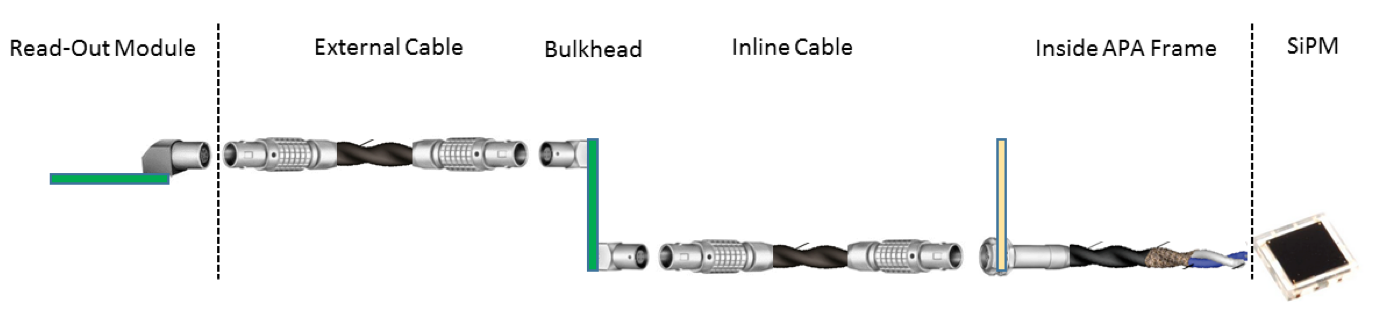
\includegraphics[width=1.0\columnwidth]{cable_plant.png}
\end{cdrfigure}

Following this step, five PDs will be inserted into the APA through one
side frame, with connections being made between the twisted-pair
cables and the SiPM PCB just as the readout end of the detector enters
the tube (see Figure~\ref{fig:5.8-2}).  The PD is then inserted the last 10~cm into
the frame, and affixed to the inner surface of the APA tube (see
Figure~\ref{fig:5.8-3}).  The process is then completed for the five PDs to be
inserted from the opposite side.

\begin{cdrfigure}[Connection between the PD twisted-pair cable and
    SiPM mounting board.]{fig:5.8-2}{Connection between the PD twisted-pair cable and SiPM mounting board.}
  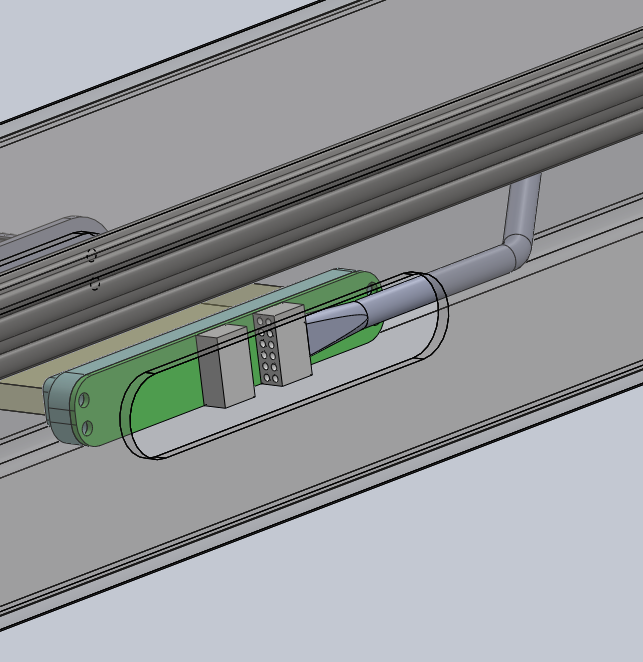
\includegraphics[width=0.6\columnwidth]{pd_frame_connector.png}
\end{cdrfigure}

\begin{cdrfigure}[Insertion of one PD paddle]{fig:5.8-3}{Insertion of one PD paddle}
  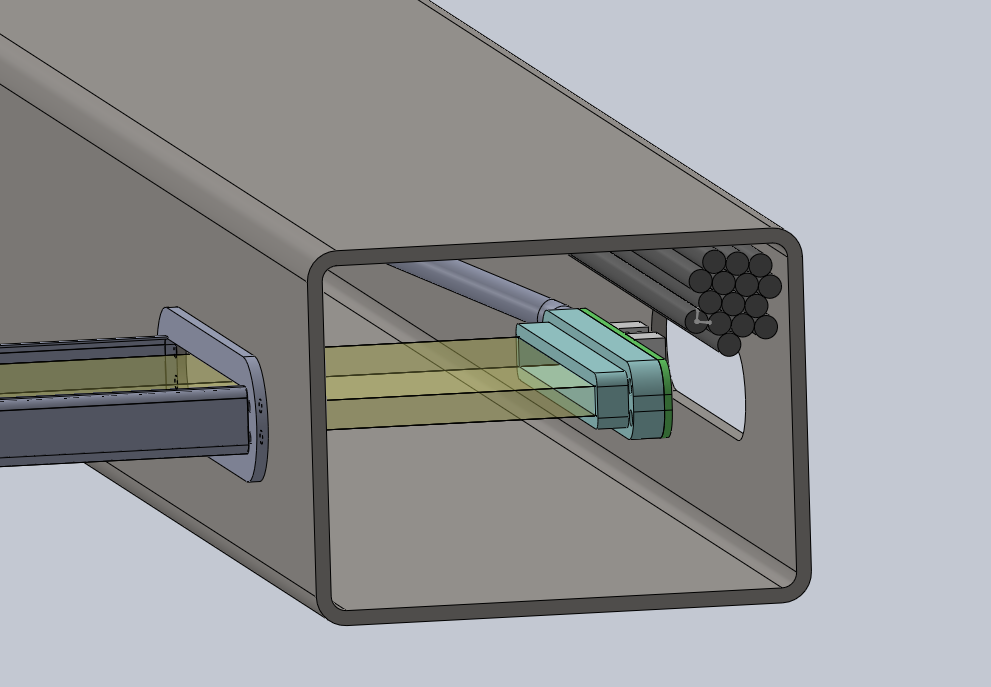
\includegraphics[width=0.6\columnwidth]{pd_insertion.png} 
\end{cdrfigure}

Following insertion of the PDs, the environmental controls required
for the PD WLS materials (UV filtering, temperature and humidity
control) will need to be observed for the entire APA.






